% ============================================================================
%  memoria.tex -- Documento principal
%  Compilar DESDE LA CARPETA memoria/ con:   pdflatex memoria   (dos veces)
%  Necesita que existan, junto a esta carpeta, las carpetas ../codigo (para
%  los listados) y las subcarpetas tablas/ y figuras/ (generadas por
%  ../experimentos/generar_tablas.py).
% ============================================================================
\documentclass[11pt,a4paper]{article}

\usepackage[utf8]{inputenc}
\usepackage[T1]{fontenc}
\usepackage{lmodern}
\usepackage[a4paper,margin=2.3cm]{geometry}

% --- Idioma: si esta instalado el paquete de espanol de babel se usa; si no,
% --- se traducen a mano los rotulos y el documento compila igualmente.
\IfFileExists{spanish.ldf}{%
  \usepackage[spanish,es-tabla,es-nodecimaldot,es-noshorthands]{babel}%
}{%
  \AtBeginDocument{%
    \renewcommand{\contentsname}{Índice}%
    \renewcommand{\figurename}{Figura}%
    \renewcommand{\tablename}{Tabla}%
    \renewcommand{\refname}{Referencias}%
    \renewcommand{\abstractname}{Resumen}%
    \renewcommand{\appendixname}{Apéndice}%
  }%
  \hyphenpenalty=10000 \exhyphenpenalty=10000 \emergencystretch=3em
}

\usepackage{amsmath,amssymb}
\usepackage{graphicx}
\usepackage{booktabs}
\usepackage{array}
\usepackage{longtable}
\usepackage{float}
\usepackage{enumitem}
\usepackage{xcolor}
\usepackage{caption}
\usepackage{tikz}
\usepackage[most]{tcolorbox}
\usepackage{listings}
\usepackage{algorithm}
\usepackage{algpseudocode}
\usepackage[hidelinks]{hyperref}

\captionsetup{font=small,labelfont=bf}
\setlist{itemsep=2pt,topsep=4pt}
\setlength{\parskip}{4pt plus 1pt}

% --- Pseudocodigo en espanol -------------------------------------------------
\floatname{algorithm}{Algoritmo}
\algrenewcommand\algorithmicwhile{\textbf{mientras}}
\algrenewcommand\algorithmicdo{\textbf{hacer}}
\algrenewcommand\algorithmicend{\textbf{fin}}
\algrenewcommand\algorithmicif{\textbf{si}}
\algrenewcommand\algorithmicthen{\textbf{entonces}}
\algrenewcommand\algorithmicelse{\textbf{si no}}
\algrenewcommand\algorithmicfor{\textbf{para}}
\algrenewcommand\algorithmicforall{\textbf{para cada}}
\algrenewcommand\algorithmicrepeat{\textbf{repetir}}
\algrenewcommand\algorithmicuntil{\textbf{hasta que}}
\algrenewcommand\algorithmicreturn{\textbf{devolver}}
\algrenewcommand\algorithmicrequire{\textbf{Entrada:}}
\algrenewcommand\algorithmicensure{\textbf{Salida:}}
\algrenewcommand{\algorithmiccomment}[1]{\hfill{\footnotesize\color{black!60}$\triangleright$ #1}}

% --- Listados de codigo C ----------------------------------------------------
\definecolor{fondo}{gray}{0.965}
\definecolor{coment}{rgb}{0.15,0.42,0.22}
\definecolor{clave}{rgb}{0.10,0.20,0.60}
\lstset{
  language=C,
  basicstyle=\ttfamily\fontsize{7.3}{8.7}\selectfont,
  keywordstyle=\color{clave}\bfseries,
  commentstyle=\color{coment},
  stringstyle=\color{black!70},
  numbers=left, numberstyle=\tiny\color{black!45}, numbersep=5pt,
  backgroundcolor=\color{fondo},
  frame=single, rulecolor=\color{black!20},
  columns=fullflexible, keepspaces=true,
  showstringspaces=false, breaklines=true, tabsize=4,
  xleftmargin=1.6em, framexleftmargin=1.4em,
  aboveskip=6pt, belowskip=6pt
}
% \fragmento{fichero}{primera}{ultima}: muestra unas lineas concretas del codigo
\newcommand{\fragmento}[3]{\lstinputlisting[firstline=#2,lastline=#3,firstnumber=#2,
  title={\footnotesize\ttfamily codigo/\detokenize{#1}, líneas #2--#3}]{../codigo/#1}}

% --- Cajas -------------------------------------------------------------------
\newtcolorbox{idea}[1][Idea clave]{breakable,colback=blue!3,colframe=blue!45!black,
  fonttitle=\bfseries\small,title={#1},left=5pt,right=5pt,top=3pt,bottom=3pt,boxrule=0.5pt}
\newtcolorbox{decision}[1][Decisión de diseño]{breakable,colback=orange!5,colframe=orange!60!black,
  fonttitle=\bfseries\small,title={#1},left=5pt,right=5pt,top=3pt,bottom=3pt,boxrule=0.5pt}
\newtcolorbox{apuntes}[1][Esquema de los apuntes]{breakable,colback=black!3,colframe=black!55,
  fonttitle=\bfseries\small,title={#1},left=5pt,right=5pt,top=3pt,bottom=3pt,boxrule=0.5pt}

% --- Abreviaturas ------------------------------------------------------------
\newcommand{\cod}[1]{\texttt{#1}}
\newcommand{\rpd}{\mathrm{RPD}}
\newcommand{\D}[1]{\Delta_{#1}}
\newcommand{\Om}[1]{\Omega_{#1}}

\title{\textbf{Metaheurísticas para el Problema de Cubrimiento}\\[4pt]
\large Memoria técnica: teoría, algoritmos, código en C\\ y calibración de parámetros}
\author{Técnicas Avanzadas de Optimización\\[2pt] {\normalsize [Nombre y apellidos]}}
\date{Noviembre de 2026}

\begin{document}
\maketitle

\begin{abstract}
\noindent Este documento explica, partiendo de cero, los algoritmos que pide la práctica para
el Problema de Cubrimiento de Conjuntos: un algoritmo constructivo, una búsqueda local y
cinco metaheurísticas (Temple Simulado, Búsqueda Tabú, GRASP, Algoritmo Genético y Búsqueda
en Entorno Variable). Para cada uno se da la idea, el esquema de los apuntes de la
asignatura, cómo se ha adaptado al problema, por qué se ha tomado cada decisión y cómo está
escrito en C. Después se describe el protocolo experimental (qué instancias se usan para
calibrar y cuáles para validar, y por qué), la calibración de todos los parámetros y la
validación de las configuraciones elegidas. Todas las cifras del documento se generan
automáticamente a partir de los ficheros de resultados que acompañan al código.
\end{abstract}

\tableofcontents
\newpage

% ============================================================================
\section{Introducción}
% ============================================================================

\subsection{Qué pide la práctica}

El enunciado plantea el \emph{problema de cubrimiento}
\[
  \min\ \{\, z = c^{\top}x \;\mid\; Ax \ge \mathbf{1},\ x \text{ binaria} \,\}
\]
con una matriz $A$ de $m$ filas y $n$ columnas y un vector de costes $c$, cuyos datos están
en los ficheros \cod{SCPXX.dat}, y pide implementar:
\begin{enumerate}
  \item un algoritmo \textbf{constructivo} y uno de \textbf{búsqueda local};
  \item las metaheurísticas \textbf{Temple Simulado} y \textbf{Búsqueda Tabú};
  \item las metaheurísticas \textbf{GRASP} y \textbf{Algoritmo Genético};
  \item una metaheurística de \textbf{Búsqueda en Entorno Variable} (VNS);
  \item un informe con los algoritmos, el código, la \textbf{calibración de los parámetros},
        las pruebas con las instancias y el análisis de los resultados.
\end{enumerate}

Esta memoria cubre los algoritmos, el código y la calibración (incluida la validación de la
calibración). El informe final de resultados y la presentación se apoyarán en ella.

\subsection{Qué se entrega}

\begin{center}
\begin{tabular}{@{}lp{11.2cm}@{}}
\toprule
Carpeta & Contenido \\ \midrule
\cod{codigo/} & Programa en C (diez ficheros), comentado línea a línea, y el guion
                \cod{compilar.sh} para compilarlo. Un único ejecutable, \cod{scp}, contiene
                los siete algoritmos. \\
\cod{experimentos/} & Guiones en Python que \emph{solo} lanzan el ejecutable muchas veces y
                recogen lo que devuelve (los algoritmos están íntegramente en C), junto con
                todos los ficheros de resultados. \\
\cod{memoria/} & Este documento en \LaTeX{} y las tablas y figuras que se generan a partir de
                los resultados. \\
\cod{datos/} & Las 6 instancias usadas para \textbf{calibrar}. \\
\cod{Validacion\_datos/} & Las 24 instancias usadas para \textbf{validar}. \\
\bottomrule
\end{tabular}
\end{center}

\subsection{Cómo leer este documento}

El documento está escrito para alguien que no conoce de antemano ni las metaheurísticas ni el
lenguaje C. Por eso sigue siempre el mismo orden:
\begin{itemize}
  \item La sección~\ref{sec:problema} explica el problema y las instancias.
  \item La sección~\ref{sec:conceptos} da el vocabulario mínimo (solución, entorno, óptimo
        local, intensificar y diversificar) que se usa en todo lo demás.
  \item La sección~\ref{sec:programa} describe las piezas del programa que comparten todos
        los algoritmos. Conviene leerla antes que las siguientes.
  \item Las secciones~\ref{sec:constructivo} a~\ref{sec:vns} dedican un apartado a cada
        algoritmo con la misma estructura: \emph{idea}, \emph{esquema de los apuntes},
        \emph{adaptación al problema} (con la justificación de cada decisión),
        \emph{parámetros} y \emph{recorrido por el código}.
  \item Las secciones~\ref{sec:metodologia} a~\ref{sec:validacion} explican cómo se han
        elegido los valores de los parámetros y cómo se ha comprobado que la elección es
        buena. Ahí se responde con detalle a la pregunta de \emph{qué instancias se usan para
        calibrar y cuáles para validar}.
  \item El apéndice contiene el código completo.
\end{itemize}

Tres tipos de recuadro ayudan a localizar lo importante:

\begin{idea}
Resume en dos o tres frases la idea que hay que retener.
\end{idea}
\begin{apuntes}
Reproduce el esquema del algoritmo tal como aparece en los apuntes de la asignatura. El
código sigue ese esquema paso a paso.
\end{apuntes}
\begin{decision}
Explica una decisión que los apuntes dejan abierta (porque depende del problema) y por qué se
ha resuelto de esa manera.
\end{decision}

\paragraph{Convenio numérico.} Los decimales se escriben con punto (4.13 y no 4,13) porque
así los escribe el programa y así aparecen en los ficheros de resultados.

% ============================================================================
\section{El problema de cubrimiento}\label{sec:problema}
% ============================================================================

\subsection{Enunciado y formulación}

Se tiene una lista de $m$ \emph{elementos} que hay que atender y una lista de $n$
\emph{recursos} entre los que elegir. Cada recurso $j$ tiene un coste $c_j$ y atiende a unos
cuantos elementos. Hay que elegir un conjunto de recursos de coste total mínimo de forma que
\textbf{todos} los elementos queden atendidos por al menos un recurso elegido.

El ejemplo clásico es la localización de servicios de emergencia: los elementos son barrios,
los recursos son posibles emplazamientos de un parque de bomberos, y un emplazamiento
``cubre'' los barrios a los que llega en menos de diez minutos. Otro ejemplo muy importante
en la práctica es la planificación de tripulaciones de aerolíneas y ferrocarriles: los
elementos son los vuelos o trayectos y cada recurso es un turno de trabajo posible.

En forma matricial, los elementos son las \textbf{filas} y los recursos las \textbf{columnas}
de una matriz $A$ de ceros y unos, con $a_{ij}=1$ si la columna $j$ cubre la fila $i$. La
variable $x_j$ vale 1 si se elige la columna $j$ y 0 si no:
\begin{equation}\label{eq:scp}
\begin{aligned}
 \min\quad & z=\sum_{j=1}^{n} c_j x_j \\
 \text{sujeto a}\quad & \sum_{j=1}^{n} a_{ij} x_j \ \ge\ 1 \qquad i=1,\dots,m \\
 & x_j\in\{0,1\} \qquad j=1,\dots,n .
\end{aligned}
\end{equation}
La restricción $i$ dice exactamente ``la fila $i$ está cubierta por al menos una columna
elegida''. En inglés el problema se llama \emph{Set Covering Problem} (SCP).

A lo largo del documento se usa este vocabulario:
\begin{itemize}
  \item una \textbf{solución} es un conjunto $S$ de columnas;
  \item es \textbf{factible} si cubre todas las filas;
  \item su \textbf{coste} es $z(S)=\sum_{j\in S} c_j$;
  \item una columna de $S$ es \textbf{redundante} si al quitarla la solución sigue siendo
        factible (todas sus filas están cubiertas también por otra columna de $S$). Quitar
        una columna redundante siempre abarata la solución, así que una buena solución no
        tiene ninguna.
\end{itemize}

\subsection{El ejemplo del enunciado}\label{sec:ejemplo}

El enunciado da un ejemplo con $m=3$ filas, $n=5$ columnas y costes $c=(2,5,4,3,1)$:
\[
A=\begin{pmatrix}
1&0&0&1&0\\
0&1&0&1&1\\
0&1&1&0&0
\end{pmatrix}
\qquad
\begin{array}{l}
\text{fila 1: la cubren las columnas 1 y 4}\\
\text{fila 2: la cubren las columnas 2, 4 y 5}\\
\text{fila 3: la cubren las columnas 2 y 3}
\end{array}
\]
La solución $\{4,3\}$ es factible (la columna 4 cubre las filas 1 y 2, la 3 cubre la fila 3)
y cuesta $3+4=7$. La solución $\{1,5,3\}$ también cuesta $2+1+4=7$. No hay ninguna más
barata, de modo que el óptimo es $z^\ast=7$. En cambio $\{4,2\}$ es factible pero cuesta 8, y
$\{1,5\}$ no es factible porque deja sin cubrir la fila 3. Este ejemplo se volverá a usar
para seguir a mano el algoritmo constructivo (sección~\ref{sec:constructivo}).

\subsection{Formato de los ficheros}

El fichero \cod{SCPXX.dat} contiene, en este orden: $m$ y $n$; los $n$ costes; y, para cada
fila, cuántas columnas la cubren seguido de los índices de esas columnas (numeradas desde 1).
Es el mismo formato de la biblioteca de problemas OR-Library de
Beasley~\cite{orlib}. El ejemplo anterior se escribe así:
\begin{verbatim}
   3 5
   2 5 4 3 1
   2
   1 4
   3
   2 4 5
   2
   2 3
\end{verbatim}
Obsérvese que el fichero describe la matriz \emph{por filas}. Los algoritmos necesitan
también la descripción \emph{por columnas} (qué filas cubre cada columna); el programa la
construye al leer (sección~\ref{sec:estructuras}).

\subsection{Por qué hacen falta heurísticas}

El problema de cubrimiento es \textbf{NP-duro}: su versión de decisión es uno de los
problemas NP-completos clásicos (los apuntes citan ``recubrimiento y empaquetado'' entre los
ejemplos de la clase NP-completo). Esto significa que no se conoce ningún algoritmo que
garantice encontrar el óptimo en un tiempo que crezca de forma polinómica con el tamaño del
problema, y se sospecha que no existe. Con $n=10\,000$ columnas hay $2^{10\,000}$
subconjuntos posibles; enumerarlos es impensable.

Los apuntes distinguen dos formas de atacar un problema así:
\begin{itemize}
  \item un \textbf{algoritmo exacto} garantiza el óptimo, pero puede necesitar un tiempo
        excesivo;
  \item un \textbf{algoritmo heurístico} da una buena solución factible en un tiempo
        razonable, sin garantía de que sea la óptima.
\end{itemize}
La práctica trata de los segundos.

\subsection{Las instancias de la práctica}\label{sec:instancias}

Se dispone de 30 instancias, \cod{SCP01} a \cod{SCP30}, todas con la misma forma. La
tabla~\ref{tab:instancias} resume sus características, medidas sobre los 30 ficheros.

\begin{table}[H]
\centering
\caption{Características de las 30 instancias (mínimo, media y máximo entre instancias).}
\label{tab:instancias}
\begin{tabular}{@{}lrrr@{}}
\toprule
Característica & Mínimo & Media & Máximo \\ \midrule
Filas $m$ & 500 & 500 & 500 \\
Columnas $n$ & 10\,000 & 10\,000 & 10\,000 \\
Unos de la matriz $A$ & 75\,021 & 75\,512 & 76\,322 \\
Densidad de $A$ (\% de unos) & 1.50 & 1.51 & 1.53 \\
Columnas que cubren a una fila & 104 & 151 & 200 \\
Filas que cubre una columna & 0 & 7.55 & 33 \\
Coste de una columna & 0.01 & 5.92 & 26.46 \\
Correlación entre coste y n.º de filas cubiertas & 0.62 & 0.66 & 0.69 \\
\bottomrule
\end{tabular}
\end{table}

De la tabla se deducen tres hechos que condicionan el diseño:
\begin{enumerate}
  \item \textbf{La matriz es muy dispersa} (solo un 1.5\,\% de unos). Guardarla como una
        tabla de $500\times 10\,000$ y recorrerla entera sería un derroche; conviene guardar
        solo los unos (sección~\ref{sec:estructuras}).
  \item \textbf{Los costes son números reales distintos entre sí}. No es un problema de
        ``coste unitario'' en el que solo importe cuántas columnas se eligen.
  \item \textbf{Las columnas caras cubren más filas} (correlación de 0.66). Elegir siempre la
        columna más barata, o siempre la que más cubre, será mala idea; hay que mirar la
        relación entre ambas cosas (sección~\ref{sec:constructivo}).
\end{enumerate}

\subsection{El valor óptimo de cada instancia}\label{sec:optimos}

Para saber si un heurístico es bueno hay que compararlo con algo. Lo ideal es compararlo con
el \emph{valor óptimo}. Aunque el problema es NP-duro en general, estas 30 instancias en
concreto resultan fáciles para un resolutor exacto de programación entera: con el resolutor
libre HiGHS (a través de la función \cod{milp} de la biblioteca SciPy~\cite{scipymilp}) cada
una se resuelve hasta optimalidad demostrada en menos de dos segundos. El guion
\cod{experimentos/calcular\_optimos.py} hace ese cálculo y el fichero
\cod{experimentos/optimos.csv} guarda los 30 valores, que van de 321.77 a 391.25.

\begin{decision}[Decisión: medir contra el óptimo exacto]
Los óptimos se usan \textbf{exclusivamente como vara de medir}. Ningún algoritmo de la
práctica los conoce ni los utiliza. La ventaja frente a comparar con ``la mejor solución
encontrada por nuestros propios algoritmos'' es que la medida es absoluta: un 4\,\% significa
de verdad un 4\,\% por encima de lo mejor posible.
\end{decision}

Al calcular los óptimos aparecen dos regularidades que conviene conocer porque explican
buena parte de los resultados:
\begin{itemize}
  \item En las 30 instancias la solución óptima tiene \textbf{exactamente 50 columnas}, es
        decir, usa columnas ``grandes'' que cubren unas 10 filas cada una.
  \item En las 30 instancias la relajación lineal del modelo~\eqref{eq:scp} (cambiar
        $x_j\in\{0,1\}$ por $0\le x_j\le 1$) tiene el mismo valor que el problema entero. Por
        eso un resolutor exacto las liquida tan deprisa.
\end{itemize}
Ambas cosas indican que las instancias se generaron escondiendo dentro una solución muy buena
de 50 columnas, rodeada de otras 9\,950 columnas ``de relleno''. Para un heurístico eso es
una trampa: como se verá, las soluciones que construye de forma natural usan unas 140--170
columnas pequeñas y baratas, que se parecen muy poco a la solución escondida. La
sección~\ref{sec:conclusiones} vuelve sobre este punto.

% ============================================================================
\section{Conceptos generales}\label{sec:conceptos}
% ============================================================================

Esta sección reúne el vocabulario de los apuntes que se usa en el resto del documento.

\subsection{Heurísticas y metaheurísticas}

Los apuntes dan estas dos definiciones:
\begin{itemize}
  \item \textbf{Heurística}: procedimiento simple, a menudo basado en el sentido común, que
        se supone que obtendrá una buena solución (factible, aunque no necesariamente
        óptima) de un problema difícil de un modo sencillo y rápido.
  \item \textbf{Metaheurística}: procedimiento iterativo maestro que guía y modifica las
        operaciones de una heurística subordinada (o varias) para producir eficientemente
        soluciones de alta calidad.
\end{itemize}
Es decir, una metaheurística no es un algoritmo para un problema concreto sino una
\emph{receta general} (``acepta de vez en cuando soluciones peores'', ``prohíbe deshacer lo
que acabas de hacer'', ``cruza soluciones buenas'') que hay que \emph{adaptar} a cada
problema. Por eso, en cada una de las cinco metaheurísticas de la práctica hay dos partes:
el esquema general, que viene de los apuntes, y las decisiones de adaptación al problema de
cubrimiento, que son nuestras y hay que justificar.

Entre las heurísticas ``simples'' los apuntes distinguen, entre otras:
\begin{itemize}
  \item \textbf{Métodos constructivos}: crean una solución paso a paso, desde la nada,
        tomando en cada paso la mejor elección según algún criterio.
  \item \textbf{Métodos de búsqueda local}: parten de una solución y la mejoran
        progresivamente mediante pequeños cambios, hasta que no se puede mejorar más.
\end{itemize}
Son los dos primeros algoritmos que pide la práctica y, además, son las piezas con las que
se montan las metaheurísticas.

\subsection{Movimiento, entorno y óptimo local}

\begin{itemize}
  \item Un \textbf{movimiento} es un cambio pequeño que transforma una solución en otra. En
        el cubrimiento, por ejemplo: quitar una columna, o cambiar una columna por otra.
  \item El \textbf{entorno} (o vecindario) de una solución $S$ es el conjunto de soluciones
        que se alcanzan con \emph{un} movimiento; sus elementos son las \textbf{vecinas} de
        $S$. Una \textbf{estructura de entornos} es la regla que dice qué movimientos se
        permiten. Con otra regla, las vecinas son otras.
  \item Una solución es un \textbf{óptimo local} respecto de una estructura de entornos si
        ninguna de sus vecinas es mejor que ella. El \textbf{óptimo global} es la mejor
        solución de todas.
\end{itemize}

\begin{figure}[H]
\centering
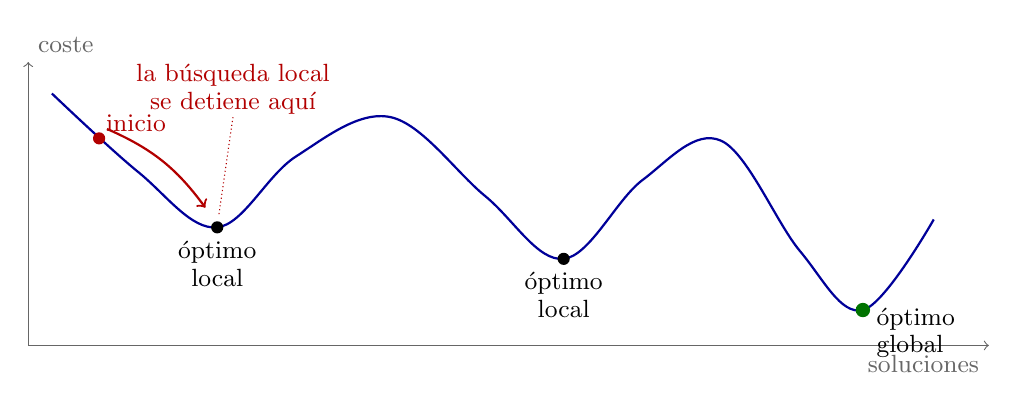
\begin{tikzpicture}[x=1cm,y=1cm]
  \draw[->,black!60] (0,0) -- (12.2,0) node[below left] {\small soluciones};
  \draw[->,black!60] (0,0) -- (0,3.6) node[above right] {\small coste};
  \draw[thick,blue!60!black] plot[smooth,tension=0.6] coordinates
     {(0.3,3.2) (1.4,2.2) (2.4,1.5) (3.4,2.4) (4.6,2.9) (5.8,1.9) (6.8,1.1) (7.8,2.1)
      (8.8,2.6) (9.8,1.2) (10.6,0.45) (11.5,1.6)};
  \fill[red!70!black] (0.9,2.63) circle (2.2pt) node[above right=-1pt] {\small inicio};
  \fill (2.4,1.5) circle (2.2pt);
  \node[below,align=center] at (2.4,1.45) {\small óptimo\\[-2pt]\small local};
  \fill (6.8,1.1) circle (2.2pt);
  \node[below,align=center] at (6.8,1.05) {\small óptimo\\[-2pt]\small local};
  \fill[green!45!black] (10.6,0.45) circle (2.6pt);
  \node[below right,align=left] at (10.65,0.6) {\small óptimo\\[-2pt]\small global};
  \draw[->,red!70!black,thick] (1.0,2.75) to[bend left=15] (2.25,1.75);
  \node[red!70!black,align=center] at (2.6,3.25) {\small la búsqueda local\\[-2pt]\small se detiene aquí};
  \draw[red!70!black,densely dotted] (2.6,2.9) -- (2.42,1.65);
\end{tikzpicture}
\caption{Una búsqueda local baja hasta el óptimo local más cercano y ahí se queda, aunque
haya soluciones mejores más lejos. Las metaheurísticas son distintas maneras de salir de ese
valle.}
\label{fig:paisaje}
\end{figure}

La figura~\ref{fig:paisaje} muestra la limitación fundamental de la búsqueda local: se
detiene en el primer óptimo local que encuentra. Las cinco metaheurísticas de la práctica son
cinco respuestas distintas a la pregunta \emph{¿cómo salgo de un óptimo local?}:

\begin{center}
\begin{tabular}{@{}lp{11cm}@{}}
\toprule
Metaheurística & Cómo escapa del óptimo local \\ \midrule
Temple Simulado & Acepta a veces movimientos que empeoran, con una probabilidad que va
                  disminuyendo. \\
Búsqueda Tabú & Hace siempre el mejor movimiento aunque empeore, y \emph{prohíbe} deshacer
                  los movimientos recientes para no volver atrás. \\
GRASP & No intenta escapar: vuelve a empezar desde otra solución inicial distinta, construida
                  con algo de azar. \\
Algoritmo Genético & Trabaja con muchas soluciones a la vez y las combina entre sí. \\
VNS & Cambia de estructura de entornos y da ``saltos'' cada vez mayores. \\
\bottomrule
\end{tabular}
\end{center}

\subsection{Intensificar y diversificar}

Todo buen heurístico tiene que equilibrar dos tendencias opuestas:
\begin{itemize}
  \item \textbf{Intensificar}: explotar a fondo la zona donde se han encontrado buenas
        soluciones (buscar cerca de lo mejor que se conoce).
  \item \textbf{Diversificar}: explorar zonas nuevas, alejadas de lo ya visitado.
\end{itemize}
Si solo se intensifica, el algoritmo se estanca enseguida; si solo se diversifica, es una
búsqueda al azar. Casi todos los parámetros que se calibran en la
sección~\ref{sec:calibracion} regulan precisamente este equilibrio (la temperatura del
temple, la duración tabú, el tamaño de la lista de candidatos de GRASP, la probabilidad de
mutación del genético o el tamaño del salto de la VNS).

\subsection{Clasificación}

Los apuntes clasifican las metaheurísticas en \textbf{trayectoriales} (manejan una única
solución que va cambiando: describe una trayectoria) y \textbf{poblacionales} (manejan un
conjunto de soluciones). De las cinco de la práctica, el Temple Simulado, la Búsqueda Tabú,
GRASP y la VNS son trayectoriales; el Algoritmo Genético es poblacional.

Como lectura complementaria general, gratuita y escrita para no especialistas, se recomienda
el libro de Luke~\cite{luke}, que figura en la bibliografía de los apuntes.

% ============================================================================
\section{Diseño común del programa}\label{sec:programa}
% ============================================================================

Los siete algoritmos están en un único programa en C. Esta sección explica las piezas que
comparten, porque casi todas las decisiones de eficiencia están aquí.

\subsection{Organización en ficheros}

\begin{center}
\begin{tabular}{@{}lp{11.5cm}@{}}
\toprule
Fichero & Contenido \\ \midrule
\cod{scp.h} & Cabecera: define los tipos de datos (instancia, solución, parámetros) y declara
              todas las funciones. No contiene código ejecutable. \\
\cod{base.c} & Herramientas comunes: números aleatorios, reloj, lectura del fichero,
              operaciones sobre una solución, \cod{completar} y \cod{perturbar}. \\
\cod{constructivo.c} & Algoritmo constructivo voraz. \\
\cod{busqueda\_local.c} & Estructuras de entornos $\D1,\D2,\D3$ y búsqueda local (VND). \\
\cod{temple.c} & Temple Simulado. \\
\cod{tabu.c} & Búsqueda Tabú. \\
\cod{grasp.c} & GRASP. \\
\cod{genetico.c} & Algoritmo Genético. \\
\cod{vns.c} & Búsqueda en Entorno Variable. \\
\cod{main.c} & Programa principal: lee los argumentos, llama al algoritmo pedido, comprueba
              la solución y escribe el resultado. \\
\bottomrule
\end{tabular}
\end{center}

\begin{decision}[Decisión: un fichero por algoritmo y un único ejecutable]
Separar cada algoritmo en su fichero permite leerlos de forma independiente. Reunirlos en un
solo ejecutable garantiza que todos usan \emph{exactamente} las mismas rutinas de lectura,
de evaluación y de medida del tiempo, de modo que las comparaciones entre ellos son justas.
\end{decision}

\subsection{Cómo se guarda la instancia}\label{sec:estructuras}

Como solo el 1.5\,\% de la matriz son unos, se guardan dos listas compactas de unos:
\begin{itemize}
  \item \textbf{por filas}: para cada fila $i$, las columnas que la cubren. Sirve para
        responder a ``¿quién puede cubrir esta fila?'';
  \item \textbf{por columnas}: para cada columna $j$, las filas que cubre. Sirve para
        responder a ``¿qué pasa si añado o quito esta columna?''.
\end{itemize}
Cada lista se guarda en dos vectores: uno con todos los índices seguidos y otro que dice
dónde empieza cada fila (o columna). Para el ejemplo de la sección~\ref{sec:ejemplo},
numerando desde 0 como se hace dentro del programa:

\begin{center}
\small
\begin{tabular}{@{}ll@{}}
\toprule
Por filas & Por columnas \\ \midrule
\cod{fila\_col = [0,3,\ 1,3,4,\ 1,2]} & \cod{col\_fil = [0,\ 1,2,\ 2,\ 0,1,\ 1]} \\
\cod{fila\_ini = [0, 2, 5, 7]} & \cod{col\_ini = [0, 1, 3, 4, 6, 7]} \\
\bottomrule
\end{tabular}
\end{center}
Así, las columnas de la fila 1 (la segunda) son \cod{fila\_col[2..4]} $=\{1,3,4\}$, es decir,
las columnas 2, 4 y 5 del enunciado. Este formato se conoce como CSR/CSC y es el habitual
para matrices dispersas.

Además se guarda la matriz completa como una tabla de bytes ($500\times10\,000=5$~MB), que
permite preguntar al instante ``¿cubre la columna $j$ la fila $i$?'' (macro \cod{CUBRE}). Solo
se usa para esa consulta puntual, nunca se recorre entera.

\fragmento{scp.h}{52}{66}

\subsection{Cómo se guarda una solución}\label{sec:solucion}

Una solución no es solo el conjunto de columnas. Se mantienen \emph{siempre actualizados}:
\begin{itemize}
  \item \cod{en[j]}: 1 si la columna $j$ está elegida;
  \item \cod{lista} y \cod{pos}: las columnas elegidas, una tras otra, y la posición de cada
        una en esa lista (permite recorrer solo las elegidas y borrar una en tiempo constante);
  \item \cod{cub[i]}: \textbf{cuántas columnas elegidas cubren la fila $i$};
  \item \cod{nsin}: cuántas filas están sin cubrir (la solución es factible si y solo si
        \cod{nsin} $=0$);
  \item \cod{z}: el coste total.
\end{itemize}

\begin{idea}[Idea clave: evaluación incremental]
Gracias al contador \cod{cub}, añadir o quitar una columna solo obliga a tocar las filas de
\emph{esa} columna (unas 7 u 8 de media), no las 500 filas ni los 75\,000 unos. Como las
metaheurísticas hacen millones de movimientos, esta es la decisión que más influye en la
velocidad del programa. También da gratis las dos preguntas que se hacen continuamente:
\emph{¿es factible?} (\cod{nsin == 0}) y \emph{¿es redundante la columna $j$?} (todas sus
filas tienen \cod{cub} $\ge 2$).
\end{idea}

\fragmento{base.c}{313}{328}

\subsection{Todas las soluciones son siempre factibles}

\begin{decision}[Decisión: no trabajar con soluciones infactibles]
Hay dos formas de tratar la restricción ``todas las filas cubiertas'': (a) permitir soluciones
que dejen filas sin cubrir y penalizarlas en la función objetivo, o (b) no salir nunca del
conjunto factible. Se ha elegido (b) en los cinco algoritmos. Razones: no hay que inventar ni
calibrar un peso de penalización; cualquier solución que el algoritmo tenga entre manos se
puede devolver tal cual; y en este problema recuperar la factibilidad es muy fácil y barato
(basta añadir columnas). Cuando un operador rompe la factibilidad (al quitar columnas, al
cruzar dos soluciones) se \textbf{repara} inmediatamente.
\end{decision}

La reparación y la construcción son, en el fondo, la misma operación: \emph{cubrir las filas
que estén sin cubrir}. Por eso existe una única función, \cod{completar}, que usan el
constructivo (partiendo de la solución vacía), GRASP, el temple, el genético y la VNS
(partiendo de una solución a la que le faltan columnas). Se explica en la
sección~\ref{sec:constructivo}.

\subsection{La perturbación \texorpdfstring{$\Om{k}$}{Omega\_k}}\label{sec:perturbar}

Varios algoritmos necesitan ``una solución parecida a $S$ elegida al azar''. Se obtiene con la
función \cod{perturbar}:
\begin{enumerate}
  \item se quitan $k$ columnas de $S$ elegidas al azar (quedan filas sin cubrir);
  \item se repara con \cod{completar}, prohibiendo que vuelvan a entrar justo las $k$ que se
        acaban de quitar;
  \item se eliminan las columnas que hayan quedado redundantes.
\end{enumerate}
Llamaremos $\Om{k}(S)$ al conjunto de soluciones que pueden salir así. Con $k$ pequeño la
nueva solución se parece mucho a $S$; con $k$ grande, poco.

\begin{decision}[Decisión: vetar las columnas recién quitadas]
Sin el veto del paso 2, el voraz volvería a meter muchas veces las mismas columnas que se
acaban de sacar (por algo estaban en la solución) y la ``vecina'' sería la propia $S$. El
veto solo dura lo que dura la reparación.
\end{decision}

\fragmento{base.c}{577}{595}

\subsection{Números aleatorios, tiempo y precisión}

\begin{itemize}
  \item \textbf{Generador aleatorio propio.} No se usa la función \cod{rand()} de C porque da
        secuencias distintas en cada sistema operativo. Se usa un generador \emph{xorshift}
        de 64 bits escrito en \cod{base.c}: con la misma semilla, el programa hace
        exactamente lo mismo en cualquier ordenador. Eso hace los experimentos
        \textbf{reproducibles} y permite depurar.
  \item \textbf{Criterio de parada por tiempo de CPU.} Todas las metaheurísticas se detienen
        al consumir un tiempo de procesador fijado (5 segundos por defecto), medido con
        \cod{clock()}. Es el criterio más justo para comparar algoritmos cuyas iteraciones
        cuestan cantidades muy distintas (una iteración del temple dura microsegundos; una
        generación del genético, milisegundos). Se mide tiempo de CPU y no de reloj para que
        no influya lo ocupado que esté el ordenador.
  \item \textbf{Tolerancia numérica.} Los costes son números reales. Para que un error de
        redondeo de $10^{-13}$ no se tome por una mejora, ``$a$ mejora a $b$'' significa
        $a<b-10^{-9}$ (constante \cod{EPS}). Además, el coste de la solución final se vuelve a
        sumar desde cero antes de escribirlo.
  \item \textbf{Comprobación independiente.} Antes de escribir el resultado,
        \cod{sol\_comprobar} recuenta desde cero la cobertura de cada fila y el coste, sin
        fiarse de los contadores. El programa solo declara una solución ``factible'' si pasa
        esa comprobación. En las 1548%
 ejecuciones de esta memoria
        la pasan todas.
\end{itemize}

% ============================================================================
\section{Algoritmo constructivo}\label{sec:constructivo}
% ============================================================================

\subsection{Idea}

Un algoritmo constructivo parte de la solución vacía y añade columnas una a una hasta que
todas las filas están cubiertas. Si en cada paso se toma la columna que \emph{en ese momento}
parece mejor, sin volver nunca atrás, el algoritmo se llama \textbf{voraz} (en inglés
\emph{greedy}). Los apuntes lo ilustran con el ``vecino más próximo'' del problema del
viajante; aquí la pregunta es qué significa ``la columna que parece mejor''.

\subsection{Tres criterios posibles}

Sea $g_j$ el número de filas \emph{todavía sin cubrir} que cubriría la columna $j$ (su
\emph{ganancia}). Hay tres criterios naturales:
\begin{center}
\begin{tabular}{@{}cll@{}}
\toprule
Criterio & Se elige la columna con\ldots & Inconveniente \\ \midrule
1 & menor coste $c_j$ & ignora cuánto cubre \\
2 & mayor ganancia $g_j$ & ignora cuánto cuesta \\
3 & mayor cociente $g_j/c_j$ & --- \\
\bottomrule
\end{tabular}
\end{center}
El criterio 3 elige la columna que cubre más filas nuevas \emph{por unidad de coste}; dicho
de otro modo, la que cubre cada fila nueva al menor precio. Es el voraz clásico del
cubrimiento (Chvátal, 1979) y tiene una garantía teórica: su solución nunca cuesta más de
$H_m = 1+\tfrac12+\dots+\tfrac1m \approx \ln m$ veces el óptimo~\cite[sec.~2.3]{kordalewski}.
En el vocabulario de los apuntes es, por tanto, un \emph{algoritmo aproximado}. En la
práctica queda muchísimo más cerca del óptimo que esa cota.

Un detalle esencial es que el criterio es \textbf{adaptativo}: $g_j$ cambia después de cada
inserción, porque las filas que se acaban de cubrir dejan de contar para las demás columnas.

\begin{algorithm}[H]
\caption{Constructivo voraz (criterio del cociente)}\label{alg:voraz}
\begin{algorithmic}[1]
\State $S\gets\emptyset$
\While{queda alguna fila sin cubrir}
  \State para cada columna $j\notin S$: $g_j\gets$ n.º de filas sin cubrir que cubre $j$
  \State $j^\ast\gets$ columna con $g_j>0$ que maximiza $g_j/c_j$
  \State $S\gets S\cup\{j^\ast\}$
\EndWhile
\State eliminar de $S$ las columnas redundantes, la más cara primero
\State \Return $S$
\end{algorithmic}
\end{algorithm}

\subsection{El paso final: quitar redundantes}

Una columna elegida al principio puede volverse innecesaria más tarde, cuando otras columnas
han cubierto todas sus filas. Por eso, al terminar, se eliminan las redundantes.

\begin{decision}[Decisión: quitar primero la redundante más cara]
Si hay varias redundantes no siempre se pueden quitar todas: dos columnas pueden ser
redundantes por separado y dejar de serlo en cuanto se quita la otra (si comparten una fila
que solo cubren ellas dos). Hay que decidir un orden. Se quita primero la más cara porque es
la que más ahorra, se recalcula, y se repite. Es, a su vez, un criterio voraz.
\end{decision}

\subsection{El algoritmo, a mano, sobre el ejemplo}

Con los datos de la sección~\ref{sec:ejemplo} ($c=(2,5,4,3,1)$) y el criterio 3:

\begin{center}
\small
\begin{tabular}{@{}clcccccl@{}}
\toprule
Paso & Filas sin cubrir & \multicolumn{5}{c}{Cociente $g_j/c_j$ de las columnas 1 a 5} & Se elige \\ \midrule
1 & 1, 2, 3 & $1/2=0.50$ & $2/5=0.40$ & $1/4=0.25$ & $2/3=0.67$ & $1/1=\mathbf{1.00}$ & columna 5 \\
2 & 1, 3 & $1/2=\mathbf{0.50}$ & $1/5=0.20$ & $1/4=0.25$ & $1/3=0.33$ & --- & columna 1 \\
3 & 3 & --- & $1/5=0.20$ & $1/4=\mathbf{0.25}$ & --- & --- & columna 3 \\
\bottomrule
\end{tabular}
\end{center}

Resultado: $S=\{5,1,3\}$, coste $1+2+4=7$, que es el óptimo. Nótese cómo cambian las
ganancias: en el paso 1 la columna 4 cubría dos filas nuevas; en el paso 2 solo una, porque
la fila 2 ya la había cubierto la columna 5. Con el criterio 2 (mayor ganancia) el mismo
algoritmo elige las columnas 4 y 2 y obtiene coste 8. Se puede comprobar con el programa:
\begin{verbatim}
   ./scp ejemplo.dat voraz criterio=3 ver=1
   ./scp ejemplo.dat voraz criterio=2 ver=1
\end{verbatim}

\subsection{Implementación: la función \cod{completar}}\label{sec:completar}

El constructivo es tan corto que cabe en tres líneas, porque todo el trabajo lo hace la
función común \cod{completar}:

\fragmento{constructivo.c}{24}{30}

\cod{completar(I, S, criterio, lrc, memoria, lambda)} cubre las filas que $S$ tenga sin
cubrir. Sus argumentos permiten usar la misma función en todos los algoritmos:
\begin{itemize}
  \item \cod{criterio}: 1, 2 o 3 (los de la tabla anterior);
  \item \cod{lrc}: tamaño de la \emph{lista restringida de candidatos}. En cada paso no se
        toma obligatoriamente la mejor columna, sino una al azar entre las \cod{lrc} mejores.
        Con \cod{lrc = 1} es el voraz puro, determinista. Con valores mayores es el voraz
        \emph{aleatorizado} que necesitan GRASP y las reparaciones (sección~\ref{sec:grasp});
  \item \cod{memoria} y \cod{lambda}: solo los usa GRASP.
\end{itemize}

El código tiene tres bloques. El primero calcula las ganancias iniciales recorriendo
únicamente las filas sin cubrir:

\fragmento{base.c}{493}{504}

El segundo, dentro del bucle principal, recorre las candidatas, descarta las que ya no
aportan nada y mantiene ordenadas las \cod{lrc} mejores (una inserción en una lista ordenada
muy corta):

\fragmento{base.c}{522}{549}

El tercero actualiza las ganancias \emph{antes} de insertar la columna elegida: por cada fila
que la elegida va a cubrir por primera vez, todas las columnas que cubren esa fila pierden
una unidad de ganancia.

\fragmento{base.c}{551}{560}

\begin{idea}[Por qué es rápido]
Las ganancias no se recalculan desde cero en cada paso: se \emph{actualizan}. Cada fila pasa
de ``sin cubrir'' a ``cubierta'' una sola vez, y en ese momento se recorre su lista de
columnas. En total se recorren los unos de la matriz como mucho una vez ($\approx 75\,000$
operaciones), más el repaso de la lista de candidatas en cada paso. Una construcción
completa tarda unos 8 milisegundos.
\end{idea}

\subsection{Comparación de los tres criterios}\label{sec:res-voraz}

La tabla~\ref{tab:basicos} (página~\pageref{tab:basicos}) recoge el resultado de los tres
criterios sobre las 30 instancias. La medida es la desviación porcentual respecto del óptimo
(RPD, definida en la sección~\ref{sec:rpd}). En las 6 instancias de calibración:
\begin{itemize}
  \item el criterio 1 (la más barata) queda un 15.9\,\% por encima del óptimo y usa unas 243
        columnas: llena la solución de columnas baratas que cubren muy poco;
  \item el criterio 2 (la que más cubre) usa solo 49 columnas pero queda un 33.4\,\% por
        encima: elige columnas grandes sin mirar que son carísimas;
  \item el criterio 3 (cociente) queda un 6.6\,\% por encima, con unas 167 columnas.
\end{itemize}

\begin{decision}[Decisión: criterio del cociente]
Se adopta el criterio 3 como constructivo de la práctica y como base de todas las
reparaciones y construcciones de las metaheurísticas. La elección se ha hecho mirando solo
las 6 instancias de calibración; las 24 de validación la confirman (6.4\,\% frente a
15.5\,\% y 31.6\,\%). Coincide con lo esperado por la estructura de las instancias (los
costes están correlacionados con la cobertura, sección~\ref{sec:instancias}).
\end{decision}

% ============================================================================
\section{Búsqueda local}\label{sec:local}
% ============================================================================

\subsection{Idea}

La búsqueda local parte de una solución factible (la del constructivo) e intenta mejorarla
con pequeños cambios. En cada paso examina las vecinas de la solución actual; si alguna es
mejor, se mueve a ella y repite; si ninguna lo es, se detiene: ha llegado a un óptimo local.
Los apuntes la describen así (transparencias de VNS): \emph{fijadas una solución inicial
$S_0$ y una estructura de entornos $E$, se examinan solo las soluciones vecinas de $E(S_0)$;
si existe $S_1$ en $E(S_0)$ mejor que $S_0$ se examina $E(S_1)$, y así sucesivamente; la
búsqueda local termina al llegar a un óptimo local.}

Todo depende, por tanto, de la estructura de entornos. Se han definido tres, de la más
pequeña a la más grande. Las tres conservan la factibilidad.

\subsection{Las tres estructuras de entornos}\label{sec:entornos}

\paragraph{$\D1$: eliminación.} Quitar una columna redundante. Es el entorno más pequeño
(como mucho tantas vecinas como columnas tiene la solución) y cualquier movimiento suyo
mejora. Es la misma operación \cod{quitar\_redundantes} del constructivo.

\paragraph{$\D2$: intercambio (1 por 1).} Sacar una columna $j$ de la solución y meter en su
lugar una columna $k$ de fuera. Para que la solución siga siendo factible, $k$ debe cubrir
todas las filas que \emph{solo} cubría $j$ (las llamaremos \textbf{filas únicas} de $j$). El
movimiento mejora si $c_k<c_j$.

\paragraph{$\D3$: inserción con expulsión (1 por $r$).} Meter una columna $k$ de fuera y
sacar \emph{todas} las columnas que, gracias a $k$, se vuelven redundantes. Pueden ser una,
dos, tres\ldots{} El valor del movimiento es
\[
  v(k) \;=\; c_k \;-\; \sum_{j\ \text{expulsada}} c_j ,
\]
y mejora la solución si $v(k)<0$. Este es el entorno que permite \emph{cambiar varias
columnas pequeñas por una grande}, que es justo lo que necesitan estas instancias (la
solución voraz tiene unas 167 columnas y la óptima 50).

\begin{decision}[Decisión: por qué estos tres entornos]
Son los movimientos más simples que conservan la factibilidad: quitar (1,0), cambiar (1,1) y
cambiar una por varias (1,$r$). No se ha incluido el movimiento ``meter dos y sacar varias''
porque su entorno tiene del orden de $n^2 = 10^8$ vecinas y no se puede explorar entero en
cada paso; ese tipo de salto más amplio se deja a las perturbaciones de las metaheurísticas.
Obsérvese que todo intercambio de $\D2$ que mejora es también un movimiento de $\D3$ (el
caso en que $k$ expulsa a una sola columna), así que $\D3$ es estrictamente más potente; la
utilidad de $\D2$ es que se explora más deprisa (solo mira las columnas que cubren una
fila concreta) y resuelve antes los casos fáciles.
\end{decision}

\subsection{Cómo se evalúa un movimiento sin ejecutarlo}

Evaluar un movimiento ``ejecutándolo, mirando el coste y deshaciéndolo'' sería lento. La
clave para hacerlo rápido son las filas únicas. La función \cod{calcular\_unicas} recorre la
solución una vez y anota:
\begin{itemize}
  \item para cada fila cubierta una sola vez, cuál es la columna que la cubre: su
        \textbf{dueña} (\cod{duena[i]});
  \item para cada columna de la solución, cuántas filas únicas tiene (\cod{nunic[j]}).
\end{itemize}

\begin{idea}[Idea clave]
Al insertar $k$, una columna $j$ de la solución se vuelve redundante \textbf{si y solo si}
$k$ cubre todas las filas únicas de $j$. Para saber a quién expulsa $k$ basta recorrer las
filas de $k$ (unas 8), mirar cuáles tienen dueña y contar cuántas filas únicas de cada dueña
cubre $k$. Si la cuenta de $j$ llega a \cod{nunic[j]}, $j$ sale.
\end{idea}

Así, evaluar la inserción de una columna cuesta lo que mide esa columna, y evaluar el entorno
$\D3$ completo (las $\approx 9\,850$ columnas de fuera) cuesta recorrer una vez los unos de
la matriz. Es lo que hace \cod{valor\_insercion}:

\fragmento{busqueda_local.c}{80}{107}

Queda un caso delicado: si $k$ vuelve redundantes a dos o más columnas, puede que no se
puedan quitar todas a la vez (si dos de ellas comparten una fila que solo cubren ellas
dos, al salir una la otra pasa a ser imprescindible). El código lo resuelve simulando: ordena las candidatas de
más cara a más barata y va sacando solo las que \emph{siguen} siendo redundantes; después
deshace la simulación. Es el mismo criterio ``la más cara primero'' del constructivo.

\fragmento{busqueda_local.c}{122}{151}

Para $\D2$ se usa un atajo distinto: como la columna que entra debe cubrir, en particular, la
\emph{primera} fila única de la que sale, solo hay que probar las columnas que cubren esa
fila (unas 150) en lugar de las 10\,000.

\fragmento{busqueda_local.c}{183}{197}

\subsection{Estrategia de exploración}

\begin{decision}[Decisión: mejor vecino]
Dentro de un entorno hay dos estrategias habituales: moverse a la \emph{primera} vecina que
mejore o evaluar todas y moverse a la \emph{mejor}. Se usa la segunda (es la que describen
los apuntes para el 2-opt: ``calcularíamos el coste de la solución obtenida con cada
intercambio y realizaríamos aquel que dé lugar a la de menor coste''). Con la evaluación
rápida de arriba, explorar el entorno entero es barato, y el resultado no depende del orden
en que se recorran las columnas, lo que hace la búsqueda determinista y reproducible.
\end{decision}

\subsection{Combinación de los entornos: búsqueda descendente (VND)}\label{sec:vnd}

Para combinar los tres entornos se usa el esquema de \emph{Búsqueda Descendente por entornos}
(VND, \emph{Variable Neighborhood Descent}) de los apuntes de VNS:

\begin{apuntes}[Esquema de los apuntes: Búsqueda Descendente (VND)]
\begin{enumerate}[label=\arabic*.,itemsep=0pt]
  \item Inicialización:
  \begin{enumerate}[label=1.\arabic*,itemsep=0pt]
    \item Construir solución inicial $S$
    \item $A=\{\D1,\dots,\D{j_A}\}$
    \item $j\gets 1$
  \end{enumerate}
  \item Repetir hasta que $j>j_A$:
  \begin{enumerate}[label=2.\arabic*,itemsep=0pt]
    \item Búsqueda local en $\D{j}$ con solución inicial $S$ $\rightsquigarrow$ $S'$
    \item Si $z(S')<z(S)$ $\Rightarrow$ $S=S'$, $j=1$; \ en otro caso $\Rightarrow$ $j=j+1$
  \end{enumerate}
  \item $S$ es mínimo local con respecto a todas las estructuras de entornos de $A$.
\end{enumerate}
\end{apuntes}

Es decir: se busca en el primer entorno hasta agotarlo; solo entonces se prueba el segundo;
y en cuanto un entorno consigue mejorar, se vuelve al primero. Al terminar, la solución es
óptimo local respecto de \emph{todos} los entornos a la vez. El código es una transcripción
literal:

\fragmento{busqueda_local.c}{268}{278}

\begin{decision}[Decisión: orden de los entornos]
Se ordenan del más barato de explorar al más caro ($\D1$, $\D2$, $\D3$). Así el entorno
caro solo se explora cuando los baratos ya no pueden hacer nada, que es la recomendación
habitual para el VND~\cite{vnsbasics}.
\end{decision}

El número de entornos $j_A$ es un parámetro (\cod{entornos}): 1, 2 o 3.

\subsection{Resultados y elección de \texorpdfstring{$j_A$}{jA}}

La ``búsqueda local'' de la práctica es: constructivo voraz + VND. La tabla~\ref{tab:basicos}
compara $j_A=1,2,3$.

\begin{table}[H]
\centering
\caption{Algoritmos básicos (deterministas): RPD medio respecto del óptimo, número medio de columnas de la solución y tiempo medio, en las 6 instancias de calibración y en las 24 de validación.}
\label{tab:basicos}
\small\setlength{\tabcolsep}{4.5pt}
\begin{tabular}{@{}lrrrrrr@{}}
\toprule
 & \multicolumn{3}{c}{Calibración (6)} & \multicolumn{3}{c}{Validación (24)} \\
\cmidrule(lr){2-4}\cmidrule(l){5-7}
Algoritmo & RPD (\%) & Columnas & $t$ (s) & RPD (\%) & Columnas & $t$ (s) \\ \midrule
Voraz, criterio 1 (menor coste) & 15.85 & 243 & 0.017 & 15.52 & 240 & 0.014 \\
Voraz, criterio 2 (mayor cobertura) & 33.43 & 49 & 0.002 & 31.61 & 49 & 0.002 \\
Voraz, criterio 3 (cociente) & 6.60 & 167 & 0.007 & 6.45 & 166 & 0.007 \\
\midrule
Búsqueda local, $j_A=1$ & 6.60 & 167 & 0.007 & 6.45 & 166 & 0.008 \\
Búsqueda local, $j_A=2$ & 6.22 & 167 & 0.010 & 6.14 & 165 & 0.008 \\
Búsqueda local, $j_A=3$ & 4.82 & 142 & 0.026 & 4.67 & 139 & 0.024 \\
\bottomrule
\end{tabular}
\end{table}


En las 6 instancias de calibración:
\begin{itemize}
  \item con $j_A=1$ el resultado es el del voraz (6.6\,\%), porque el voraz ya termina sin
        columnas redundantes;
  \item con $j_A=2$ (se añade el intercambio) baja a 6.2\,\%: mejora poco;
  \item con $j_A=3$ (se añade la inserción con expulsión) baja a 4.8\,\%, y la solución pasa
        de unas 167 columnas a unas 142. El tiempo sube de 8 a 24 milisegundos.
\end{itemize}

\begin{decision}[Decisión: $j_A=3$]
La búsqueda local de la práctica usa los tres entornos. El entorno $\D3$ es el que de verdad
aporta, y su coste en tiempo es despreciable. Como antes, la decisión se ha tomado con las 6
instancias de calibración y las 24 de validación la confirman (4.7\,\% frente a 6.1\,\%).
\end{decision}

\begin{idea}[Qué queda por hacer]
La búsqueda local tarda centésimas de segundo y se queda a un 4.7--4.8\,\% del óptimo. Las
metaheurísticas disponen de 5 segundos (unas 200 veces más tiempo): la cuestión es cuánto de
esa distancia consiguen recortar.
\end{idea}

% ============================================================================
\section{Temple Simulado}\label{sec:temple}
% ============================================================================

\subsection{Idea}

El Temple Simulado (\emph{Simulated Annealing}, Kirkpatrick, Gelatt y Vecchi, 1983) se inspira
en el templado de materiales: si un vidrio o un metal fundido se enfría muy despacio, sus
partículas tienen tiempo de colocarse en la configuración de mínima energía; si se enfría de
golpe, quedan atrapadas en una configuración peor. En la analogía, la ``energía'' es el coste
de la solución y la ``temperatura'' $T$ es un número que controla cuánto desorden se tolera.

El algoritmo es una búsqueda local con una diferencia: cuando la vecina generada es
\emph{peor} que la solución actual no se rechaza siempre, sino que se acepta con probabilidad
\[
   P(\text{aceptar}) \;=\; e^{-\delta/T}, \qquad \delta = C(y)-C(x) \ \ge 0 ,
\]
donde $\delta$ es el empeoramiento. Esta fórmula tiene dos propiedades que son toda la gracia
del método:
\begin{itemize}
  \item cuanto mayor es el empeoramiento $\delta$, menor es la probabilidad de aceptarlo;
  \item cuanto mayor es la temperatura $T$, más fácil es aceptar empeoramientos.
\end{itemize}

\begin{center}
\small
\begin{tabular}{@{}lccc@{}}
\toprule
 & $\delta=0.1$ & $\delta=1$ & $\delta=5$ \\ \midrule
$T=5$ (caliente) & 0.98 & 0.82 & 0.37 \\
$T=1$ & 0.90 & 0.37 & 0.007 \\
$T=0.1$ (frío) & 0.37 & 0.00005 & $\approx 0$ \\
\bottomrule
\end{tabular}
\end{center}

Al principio $T$ es alta y el algoritmo se pasea casi libremente por el espacio de soluciones
(\textbf{diversifica}); a medida que $T$ baja, se va pareciendo a una búsqueda local que solo
acepta mejoras (\textbf{intensifica}). Una exposición breve y rigurosa del método puede
leerse en~\cite{bertsimas}; una más informal, en~\cite[cap.~2]{luke}.

\subsection{Esquema de los apuntes}

\begin{apuntes}[Esquema de los apuntes: Temple Simulado, algoritmo general]
\begin{tabbing}
\quad\=\quad\=\quad\=\quad\=\kill
Construir una solución inicial $x\in S$ y poner $x^\ast=x$\\
Determinar la temperatura inicial $T>0$\\
Repetir \{\\
\> $n=0$\\
\> Repetir \{\\
\>\> Generar una solución vecina $y\in V(x)$\\
\>\> Evaluar $y$ calculando $\delta=C(y)-C(x)$\\
\>\> Si ($\delta<0$) [$y$ es mejor que $x$]: \ $x=y$; \ si $C(x)<C(x^\ast)$ poner $x^\ast=x$\\
\>\> Si ($\delta\ge 0$) [$y$ no es mejor que $x$]:\\
\>\>\> Generar un número aleatorio $u\in(0,1)$\\
\>\>\> Si $u<\exp(-\delta/T)$ hacer $x=y$\\
\>\> $n=n+1$\\
\> \} Mientras $n\le N(T)$\\
\> Disminuir $T$\\
\} Mientras no se haya alcanzado el criterio de parada
\end{tabbing}
\end{apuntes}

Los apuntes señalan qué hay que decidir para aplicarlo. Por un lado la \emph{adaptación al
problema}: conjunto factible, cálculo del coste, estructura de entornos y solución inicial.
Por otro la \emph{estrategia de templado}: temperatura inicial, cómo disminuye, número de
iteraciones por temperatura y criterio de parada. Los apartados siguientes responden a cada
punto.

\subsection{Adaptación al problema de cubrimiento}

\paragraph{Conjunto factible y coste.} Las soluciones son siempre coberturas factibles y el
coste es $z$ (sección~\ref{sec:programa}). Como la solución lleva su coste actualizado,
$\delta$ es una simple resta.

\paragraph{Solución inicial.} La del constructivo voraz (criterio del cociente).

\paragraph{Vecindad.} El esquema pide ``generar una solución vecina'', es decir, \emph{una
vecina al azar}, no la mejor.

\begin{decision}[Decisión: la vecina se genera con la perturbación $\Om{k}$]
La vecina de $x$ se obtiene con la función \cod{perturbar} (sección~\ref{sec:perturbar}): se
quitan $k$ columnas al azar, se reparan las filas descubiertas con el voraz aleatorizado y se
eliminan redundantes. Razones:
\begin{itemize}[itemsep=0pt]
  \item La vecina es siempre factible, como exige nuestro diseño.
  \item Un movimiento más simple no sirve como vecindad \emph{aleatoria}: si se quita una
        columna al azar la solución casi siempre deja de ser factible, y si se añade una al
        azar la solución solo empeora. Un movimiento de inserción de $\D3$ elegido al azar
        casi siempre empeora mucho, porque la mayoría de las columnas no vuelve redundante a
        ninguna otra; elegirlos al azar desperdiciaría casi todas las iteraciones.
  \item Con $\Om{k}$ la diferencia de coste $\delta$ es pequeña y puede ser positiva o
        negativa, que es lo que el temple necesita para funcionar.
  \item El tamaño del cambio se regula con un solo número, $k$.
\end{itemize}
\end{decision}

\paragraph{Temperatura inicial.} La temperatura no tiene unidades ``naturales'': un valor
bueno depende de lo grandes que sean las diferencias de coste entre vecinas, que cambian de
una instancia a otra.

\begin{decision}[Decisión: fijar $T_0$ a partir de una probabilidad $p_0$]
En lugar de calibrar $T_0$ directamente, se calibra la probabilidad $p_0$ con la que se
quiere aceptar, al empezar, un empeoramiento ``típico''. El programa genera 100 vecinas de la
solución inicial, calcula el empeoramiento medio $\bar\delta^{+}$ de las que empeoran y
despeja $T_0$ de $e^{-\bar\delta^{+}/T_0}=p_0$:
\[
   T_0 \;=\; \frac{-\,\bar\delta^{+}}{\ln p_0}.
\]
Así el parámetro tiene un significado claro (``al principio acepto la mitad de los
empeoramientos'' si $p_0=0.5$) y la temperatura se adapta sola a cada instancia.
\end{decision}

\fragmento{temple.c}{67}{83}

\paragraph{Enfriamiento.} Se usa el enfriamiento \emph{geométrico}, $T\leftarrow\alpha T$ con
$0<\alpha<1$. Es el ejemplo que dan los apuntes~\cite{yanez} (``por ejemplo, $T=\alpha T$,
$0<\alpha<1$'') y el más habitual: baja deprisa al principio (cuando casi todo se acepta y
hay poco que ganar) y cada vez más despacio después.

\paragraph{Iteraciones por temperatura.} $N(T)=L$ constante: se generan $L$ vecinas con cada
valor de la temperatura.

\paragraph{Parada y recalentamiento.} El criterio de parada es el tiempo de CPU. Puede
ocurrir que la temperatura baje tanto que ya no se acepte ningún cambio mucho antes de que se
acabe el tiempo.

\begin{decision}[Decisión: recalentar si el sistema se congela]
Si durante 5 temperaturas seguidas no se acepta ningún cambio de coste, se considera que el
sistema está congelado: la temperatura vuelve a $T_0$ y la búsqueda se reanuda desde la mejor
solución conocida $x^\ast$. Sin esto, con un enfriamiento rápido el algoritmo pasaría casi
todo el tiempo parado en un óptimo local. Volver a $x^\ast$ (y no seguir desde la solución
actual) es una forma de intensificación.
\end{decision}

\subsection{Parámetros}

\begin{center}
\begin{tabular}{@{}llp{9.6cm}@{}}
\toprule
Nombre & Símbolo & Significado y efecto \\ \midrule
\cod{k} & $k$ & Columnas que se quitan para generar una vecina. Pequeño: vecinas muy
               parecidas, pasos cortos y baratos. Grande: pasos largos y más caros. \\
\cod{lrc} & --- & Tamaño de la lista de candidatos al reparar. Con 1 la reparación es
               determinista; con más, hay más variedad de vecinas. \\
\cod{p0} & $p_0$ & Probabilidad inicial de aceptar un empeoramiento típico. Fija $T_0$. Alta:
               empieza muy ``caliente'' (explora). Baja: empieza casi como una búsqueda local. \\
\cod{alfa} & $\alpha$ & Factor de enfriamiento. Cercano a 1: enfría despacio. \\
\cod{L} & $L$ & Vecinas generadas en cada temperatura. \\
\bottomrule
\end{tabular}
\end{center}

\begin{idea}[Cómo interactúan $\alpha$, $L$ y el tiempo]
Con $k=2$ el programa genera unas 84\,000 vecinas por segundo, es decir, unas 420\,000 en los
5 segundos. Eso son $420\,000/L$ temperaturas distintas, y la temperatura final es
$T_0\,\alpha^{420\,000/L}$. Por tanto $\alpha$ y $L$ no son independientes: lo que importa es
\emph{a qué temperatura se llega cuando se acaba el tiempo}. Si se llega demasiado caliente,
el algoritmo no ha llegado a intensificar; si se enfría demasiado pronto, se pasa el tiempo
recalentando. La calibración (sección~\ref{sec:cal-temple}) lo muestra con claridad.
\end{idea}

\subsection{Recorrido por el código}

El bucle principal es una transcripción del esquema de los apuntes. Los comentarios citan la
línea del esquema a la que corresponde cada instrucción.

\fragmento{temple.c}{87}{120}

Dos detalles de implementación:
\begin{itemize}
  \item ``$x=y$'' no se hace copiando la solución, sino \emph{intercambiando} las dos
        variables (línea \cod{tmp = x; x = y; y = tmp;}). Es instantáneo.
  \item Cuando la vecina tiene exactamente el mismo coste ($\delta=0$), $e^{0}=1$ y se acepta
        siempre: el algoritmo puede desplazarse por ``mesetas'' de soluciones de igual coste.
        Esos desplazamientos no se cuentan como cambios aceptados para decidir si el sistema
        está congelado.
\end{itemize}

% ============================================================================
\section{Búsqueda Tabú}\label{sec:tabu}
% ============================================================================

\subsection{Idea}

La Búsqueda Tabú (\emph{Tabu Search}, Glover, 1986; Hansen, 1986) es una búsqueda local que
\textbf{no se detiene} al llegar a un óptimo local. En cada iteración ejecuta el mejor
movimiento disponible \emph{aunque empeore} la solución. El problema evidente es que, tras un
movimiento que empeora, el mejor movimiento siguiente sería deshacerlo, y el algoritmo
entraría en un ciclo sin fin entre dos soluciones. La solución es dotarlo de
\textbf{memoria}:

\begin{itemize}
  \item \textbf{Memoria a corto plazo (lista tabú).} Los movimientos hechos recientemente
        quedan prohibidos (son ``tabú'') durante un cierto número de iteraciones, que se
        llama \emph{duración} tabú. Así no se puede volver atrás enseguida y la búsqueda se
        ve obligada a alejarse del óptimo local.
  \item \textbf{Función de aspiración.} Una prohibición puede impedir un movimiento
        excelente. Por eso se permite saltarse el tabú si el movimiento cumple un criterio
        de aspiración; lo habitual (dicen los apuntes) es aceptarlo \emph{si mejora la mejor
        solución conocida hasta el momento}.
  \item \textbf{Memoria a largo plazo.} Se registra la \emph{frecuencia} con que se ha hecho
        cada movimiento desde el principio, y se usa para \emph{diversificar} (penalizar lo
        que se ha hecho muchas veces, para visitar zonas nuevas) o para \emph{intensificar}
        (volver a lo que ha dado buenos resultados). Según los apuntes, esto se hace
        habitualmente añadiendo a la función objetivo una penalización proporcional a la
        frecuencia del movimiento.
\end{itemize}

A diferencia del temple, la búsqueda tabú es esencialmente determinista: no decide al azar,
sino que usa la historia de la búsqueda. Un tutorial clásico y de acceso libre
es~\cite{glover}.

\subsection{Esquema de los apuntes}

\begin{apuntes}[Esquema de los apuntes: esquema de un algoritmo de búsqueda tabú]
\begin{tabbing}
\quad\=\quad\=\kill
Inicialización: \ $s\in X$; \ $s^\ast=s$; \ $k=0$; \ $T=\emptyset$; \ $A(z)=z$\\
Proceso:\\
\> \textbf{do}\\
\>\> $M(s,k)=\{\,m\in M \;/\; m\notin T \ \vee\ f(s\oplus m)<A(f(s))\,\}$ \quad (movimientos válidos)\\
\>\> $V^\ast=\{\,s'\in X \;/\; s'=s\oplus m,\ m\in M(s,k)\,\}$ \quad (conjunto de vecinos)\\
\>\> Se elige la mejor solución $s'\in V^\ast$\\
\>\> If $(f(s')<f(s^\ast))$ \ $s^\ast=s'$\\
\>\> Actualizar $T$ y $A(\cdot)$\\
\>\> $k=k+1$; \ $s=s'$\\
\> \textbf{while} (condición de parada)
\end{tabbing}
\end{apuntes}

En palabras: $s\oplus m$ es la solución que resulta de aplicar el movimiento $m$ a $s$. En
cada iteración se forma el conjunto $M(s,k)$ de movimientos \emph{válidos} (los que no están
en la lista tabú $T$, más los que sí están pero cumplen la aspiración), se ejecuta el mejor
de ellos y se actualizan la mejor solución $s^\ast$ y la lista tabú.

\subsection{Adaptación al problema de cubrimiento}

\paragraph{Movimientos.} Se necesitan movimientos que permitan tanto mejorar como empeorar de
forma controlada, manteniendo la factibilidad.

\begin{decision}[Decisión: dos tipos de movimiento simétricos]
\begin{itemize}[itemsep=1pt]
  \item \textbf{Entrada} de una columna $k$: entra $k$ y salen las columnas que $k$ vuelve
        redundantes. Es el movimiento de $\D3$. Valor: $v=c_k-\sum c_{\text{salen}}$.
  \item \textbf{Salida} de una columna $j$: sale $j$ y las filas que solo cubría ella se
        vuelven a cubrir con el voraz del cociente (entran una o varias columnas). Valor:
        $v=\sum c_{\text{entran}}-c_j$.
\end{itemize}
La entrada cambia ``varias por una'' y la salida ``una por varias''. Hacen falta las dos: con
solo entradas la búsqueda únicamente puede reducir el número de columnas y se queda sin
movimientos útiles en cuanto llega a un óptimo local de $\D3$; las salidas le permiten
desandar el camino por otro sitio. En cada iteración se valoran \emph{todos} los movimientos
de ambos tipos y se ejecuta el de menor valor admisible, sea negativo (mejora) o positivo
(empeora).
\end{decision}

\paragraph{Qué se declara tabú.} No se guardan soluciones completas (compararlas sería
carísimo), sino \emph{atributos} de los movimientos: las columnas que han entrado o salido.

\begin{decision}[Decisión: dos listas tabú, una de entrada y otra de salida]
\begin{itemize}[itemsep=1pt]
  \item Una columna que \textbf{sale} no puede volver a \textbf{entrar} durante un tiempo.
        Impide deshacer el movimiento.
  \item Una columna que \textbf{entra} no puede \textbf{salir} durante un tiempo. Impide que
        la expulsen nada más llegar, antes de que la búsqueda haya podido aprovecharla.
\end{itemize}
Cada lista tiene su propia duración (\cod{tent} y \cod{tsal}) porque no son simétricas: hay
casi 9\,900 columnas fuera de la solución y solo unas 130 dentro. Prohibir la entrada de 20
columnas apenas restringe; prohibir la salida de 20 columnas bloquea una parte apreciable de
la solución. Por eso cabe esperar que convenga $\cod{tsal}<\cod{tent}$; la calibración lo
comprueba (sección~\ref{sec:cal-tabu}).
\end{decision}

\begin{decision}[Decisión: cómo se implementa la lista tabú]
No hay una ``lista'' propiamente dicha. Para cada columna $j$ se guarda el número de la
iteración hasta la cual está prohibida: \cod{tabu\_ent[j]} y \cod{tabu\_sal[j]}. Comprobar si
un movimiento es tabú es una comparación (\cod{tabu\_ent[k] > iter}) y las prohibiciones
caducan solas, sin tener que borrar nada. Es equivalente a la ``estructura de datos tabú'' de
los apuntes, que guarda cuántas iteraciones de prohibición le quedan a cada movimiento, pero
evita tener que restar uno a todas las casillas en cada iteración.
\end{decision}

\begin{decision}[Decisión: duración aleatoria]
La duración de cada prohibición se sortea entre \cod{ten} y $2\cdot\cod{ten}$. Con una
duración fija, la búsqueda puede caer en ciclos de longitud mayor que la duración; variarla
al azar los rompe. Es la recomendación de~\cite[sec.~3.2.3]{glover}.
\end{decision}

\paragraph{Función de aspiración.} Los apuntes dan dos ejemplos, $A(z)=z$ y
$A(z)=C(x^\ast)$, y añaden que ``es habitual solo aceptar un movimiento tabú si mejora la
mejor solución conocida hasta el momento''. Se usa esta segunda, $A=f(s^\ast)$: un
movimiento tabú se admite si lleva a una solución mejor que la mejor conocida. No puede
producir ciclos (una solución mejor que todas las anteriores es, por fuerza, nueva), cosa que
$A(z)=z$ no garantiza.

\paragraph{Memoria a largo plazo: diversificación.} \cod{frec[j]} cuenta cuántas veces ha
entrado la columna $j$ en la solución. Al comparar movimientos no se usa el valor $v$ sino el
valor penalizado
\[
   v' \;=\; v \;+\; \beta\cdot\sum_{j\ \text{que entra}} \cod{frec}[j] ,
\]
de modo que, a igualdad de valor, se prefieren las columnas que se han usado poco. Es la
misma idea del ejemplo de los apuntes~\cite{yanez}, donde al valor de cada movimiento se le
resta su frecuencia absoluta (allí el problema es de máximo; aquí, de mínimo, se suma). El
peso $\beta$ es necesario porque nuestros valores son costes reales y las frecuencias son
números enteros: sin él no serían comparables. Con $\beta=0$ no hay memoria a largo plazo.

\paragraph{Intensificación.} Si pasan \cod{reinicio} iteraciones sin mejorar $s^\ast$, la
búsqueda vuelve a $s^\ast$ con las listas tabú vacías. Las frecuencias \emph{no} se borran,
así que la búsqueda no repetirá el mismo camino que la vez anterior.

\paragraph{Limpieza.} Tras un movimiento pueden quedar columnas redundantes. Se eliminan las
que no estén protegidas por el tabú de salida, y cada una queda con prohibición de volver a
entrar.

\subsection{Parámetros}

\begin{center}
\begin{tabular}{@{}lp{11.3cm}@{}}
\toprule
Nombre & Significado y efecto \\ \midrule
\cod{tent} & Duración tabú de \emph{entrada} (para las columnas que salen). Corta: riesgo de
             ciclos. Larga: se prohíben demasiadas columnas buenas. \\
\cod{tsal} & Duración tabú de \emph{salida} (para las columnas que entran). \\
\cod{beta} & Peso $\beta$ de la penalización por frecuencia. Mayor: más diversificación. \\
\cod{reinicio} & Iteraciones sin mejora antes de volver a $s^\ast$. Menor: más
             intensificación. Un valor enorme equivale a no reiniciar nunca. \\
\bottomrule
\end{tabular}
\end{center}

\subsection{Recorrido por el código}

Cada iteración empieza valorando todas las entradas. Obsérvese la condición de admisibilidad
(tabú y aspiración) y la penalización por frecuencia, que corresponden a la definición de
$M(s,k)$ del esquema:

\fragmento{tabu.c}{195}{208}

Después se valoran las salidas con \cod{valor\_salida}, que simula la reparación voraz
mirando solo las filas únicas de la columna que sale (son muy pocas), sin tocar la solución.
Elegido el mejor movimiento, se ejecuta y se actualizan las dos listas tabú y las
frecuencias (``Actualizar $T$'' en el esquema):

\fragmento{tabu.c}{245}{262}

Por último se actualiza la mejor solución y, si procede, se intensifica:

\fragmento{tabu.c}{269}{287}

\begin{idea}[Coste de una iteración]
Una iteración tabú valora casi 9\,900 entradas y unas 130 salidas, lo que supone recorrer
los unos de la matriz. El programa hace unas 950 iteraciones por segundo. Es decir, en el
mismo tiempo la búsqueda tabú da unas 90 veces menos pasos que el temple, pero cada paso es
el \emph{mejor} de unos 10\,000 movimientos y no uno al azar. Son dos formas opuestas de
gastar el tiempo de cálculo.
\end{idea}

% ============================================================================
\section{GRASP}\label{sec:grasp}
% ============================================================================

\subsection{Idea}

GRASP (\emph{Greedy Randomized Adaptive Search Procedure}, Feo y Resende, 1989) nació
precisamente para un problema de cubrimiento difícil. Su idea es la más sencilla de las
cinco: en lugar de intentar escapar de un óptimo local, \textbf{se empieza de nuevo} desde
otra solución inicial, muchas veces, y se guarda la mejor. Cada iteración tiene dos fases:
\begin{enumerate}
  \item \textbf{Fase constructiva}: se construye una solución partiendo de cero.
  \item \textbf{Fase de búsqueda local}: se mejora esa solución.
\end{enumerate}
Para que cada iteración dé una solución distinta, la construcción no puede ser el voraz
puro (que da siempre la misma). Las tres palabras del nombre describen cómo se construye
(apuntes):
\begin{itemize}
  \item \textbf{Greedy}: en cada paso se incorpora un elemento que parece adecuado según una
        medida voraz;
  \item \textbf{Randomized}: no se elige siempre el mejor según esa medida, sino que se sortea
        entre varios ``buenos'' candidatos; por ejemplo, entre los $k$ mejores;
  \item \textbf{Adaptive}: los candidatos se reevalúan cada vez que se incorpora uno.
\end{itemize}
El conjunto de buenos candidatos entre los que se sortea se llama \textbf{lista restringida
de candidatos} (LRC; en inglés RCL). Una descripción completa y de acceso libre del método y
sus variantes es~\cite{resende}.

\subsection{Esquema de los apuntes}

\begin{apuntes}[Esquema de los apuntes: GRASP, algoritmo general]
\begin{tabbing}
\quad\=\kill
Repetir \{\\
\> Construir una solución $x\in S$ de forma greedy, aleatorizada y adaptativa\\
\> Aplicar una búsqueda local a la solución $x$\\
\> Actualizar la mejor solución conocida $x^\ast$\\
\> Actualizar la información relativa a la memoria\\
\} Mientras no se haya alcanzado el criterio de parada
\end{tabbing}
\end{apuntes}

La cuarta línea (``memoria'') distingue este esquema del GRASP básico, en el que cada
iteración es independiente de las anteriores. Los apuntes dedican una transparencia a esa
\emph{memoria y guía inteligente de la construcción}: se toma como referencia un
\textbf{conjunto élite} con un número reducido de soluciones buenas y diversas, y el criterio
de construcción pasa a ser
\[
   \lambda\,[\text{greedy}] \;+\; (1-\lambda)\,[\text{memoria}] ,
\]
con $\lambda$ grande en las primeras iteraciones (aún no se sabe nada: manda el criterio
voraz), intermedio y bajando después, y pequeño en las últimas (manda la memoria).

\subsection{Adaptación al problema de cubrimiento}

\paragraph{Fase constructiva.} Es la función \cod{completar} de la
sección~\ref{sec:completar}, partiendo de la solución vacía, con el criterio del cociente
$g_j/c_j$ y una LRC de tamaño \cod{lrc}. Es \emph{greedy} (cociente), \emph{randomized}
(sorteo dentro de la LRC) y \emph{adaptive} (las ganancias $g_j$ se actualizan tras cada
inserción).

\begin{decision}[Decisión: LRC por cardinalidad]
Hay dos formas de definir la LRC: por \emph{cardinalidad} (las $k$ mejores candidatas) o por
\emph{valor} (todas las que estén a menos de un cierto porcentaje de la mejor). Se usa la
primera, que es el ejemplo de los apuntes (``se elige aleatoriamente entre los $k$ mejores
elementos''): el parámetro es un entero con un significado inmediato y la cantidad de azar es
la misma en todos los pasos de la construcción.
\end{decision}

\paragraph{Memoria.} Se mantiene un conjunto élite con las \cod{elite} mejores soluciones
\emph{distintas} encontradas. A partir de él se calcula, para cada columna,
\[
   \text{memoria}[j] \;=\; \text{fracción de soluciones élite que contienen la columna } j
   \ \in[0,1].
\]
Una columna que aparece en todas las soluciones buenas tiene memoria 1; una que no aparece en
ninguna, 0. La puntuación con la que se forma la LRC es
\begin{equation}\label{eq:grasp}
   \text{punt}(j) \;=\; \lambda\cdot\frac{g_j/c_j}{\max_k\, g_k/c_k}
                 \;+\;(1-\lambda)\cdot\text{memoria}[j].
\end{equation}

\begin{decision}[Decisión: normalizar el término voraz]
El cociente $g_j/c_j$ puede valer 0.3 o 30 según el momento de la construcción, mientras que
la memoria está siempre entre 0 y 1. Si se sumaran tal cual, $\lambda$ no significaría nada.
Dividiendo por el mejor cociente del momento, el término voraz también queda entre 0 y 1 y
$\lambda$ es de verdad ``el peso del criterio voraz''.
\end{decision}

\begin{decision}[Decisión: $\lambda$ decrece linealmente con el tiempo]
Siguiendo las tres fases que describen los apuntes, $\lambda$ empieza en $\lambda_0=1$ y baja
en línea recta hasta $\lambda_f$ cuando se agota el tiempo:
$\lambda(t)=\lambda_0+(\lambda_f-\lambda_0)\,t/t_{\max}$. Se fija $\lambda_0=1$ porque en la
primera iteración el conjunto élite está vacío y solo puede guiar el criterio voraz. El
único valor que queda por calibrar es $\lambda_f$; con $\lambda_f=1$ la memoria no se usa
nunca y el algoritmo es el GRASP básico, lo que permite medir si la memoria aporta algo.
\end{decision}

\paragraph{Actualización del conjunto élite.} Tras cada iteración, la solución obtenida
entra en el élite si no está ya (no se admiten repetidas: el élite debe ser diverso) y,
cuando está lleno, solo si mejora a la peor, a la que sustituye. Es el compromiso ``calidad
frente a diversidad'' que mencionan los apuntes.

\paragraph{Fase de búsqueda local.} El VND de la sección~\ref{sec:vnd} con \cod{grent}
entornos. Los apuntes advierten que hay que decidir ``dónde es más interesante realizar un
mayor gasto computacional: construcción o mejora''. Con dos entornos las iteraciones son más
baratas y se hacen más; con tres, cada solución queda mejor. La calibración decide.

\subsection{Parámetros}

\begin{center}
\begin{tabular}{@{}lp{11.3cm}@{}}
\toprule
Nombre & Significado y efecto \\ \midrule
\cod{lrc} & Tamaño de la LRC. Con 1 todas las construcciones serían iguales. Pequeño:
            soluciones buenas pero parecidas. Grande: soluciones variadas pero peores. \\
\cod{lamf} & Valor final $\lambda_f$ de $\lambda$. Con 1 no hay memoria (GRASP básico). Cuanto
            menor, más pesa la memoria al final. \\
\cod{elite} & Tamaño del conjunto élite. \\
\cod{grent} & Número de entornos de la búsqueda local (2 o 3). \\
\bottomrule
\end{tabular}
\end{center}

\subsection{Recorrido por el código}

Las dos fases y el cálculo de $\lambda$:

\fragmento{grasp.c}{59}{73}

Dentro de \cod{completar}, la fórmula~\eqref{eq:grasp} es una sola instrucción (la variable
\cod{vmax} es el mejor cociente del momento):

\fragmento{base.c}{527}{531}

Y la actualización de la memoria, que solo se recalcula cuando el élite cambia:

\fragmento{grasp.c}{93}{112}

% ============================================================================
\section{Algoritmo Genético}\label{sec:genetico}
% ============================================================================

\subsection{Idea}

Los algoritmos genéticos (Holland, 1975) imitan la evolución de las especies. En lugar de una
sola solución que se va modificando, se mantiene una \textbf{población} de soluciones que
evoluciona generación tras generación. El vocabulario es el de la biología:

\begin{center}
\begin{tabular}{@{}lp{11cm}@{}}
\toprule
Término & Significado en optimización \\ \midrule
Individuo & Una solución factible. \\
Gen & Cada una de las componentes con que se codifica la solución. \\
Población & El conjunto de soluciones que se mantiene en cada momento. \\
Aptitud (\emph{fitness}) & Medida de la calidad de un individuo; se deriva del coste. \\
Cruce & Operador que combina dos individuos (padres) para dar otros nuevos (hijos) que
        heredan características de ambos. \\
Mutación & Operador que altera al azar alguna característica de un individuo. \\
Selección & Operador que decide qué individuos sobreviven. \\
Generación & Una iteración del algoritmo. \\
\bottomrule
\end{tabular}
\end{center}

La apuesta del método es que \emph{combinar} soluciones buenas da, con cierta frecuencia,
soluciones aún mejores: si un padre ha resuelto bien una parte del problema y el otro otra
parte, un hijo puede heredar las dos. La mutación introduce material nuevo que el cruce por
sí solo nunca generaría, y la selección empuja a la población hacia las soluciones de menor
coste. Una introducción general gratuita es~\cite[cap.~3]{luke}.

\subsection{Esquema de los apuntes}

\begin{apuntes}[Esquema de los apuntes: Algoritmos Genéticos, algoritmo general]
\begin{tabbing}
\quad\=\kill
Construir una población inicial de soluciones\\
Guardar la mejor solución $x^\ast$\\
Repetir \{\\
\> Seleccionar progenitores y aplicar el OPERADOR DE CRUCE\\
\> Aplicar el OPERADOR DE MUTACIÓN sobre las nuevas soluciones\\
\> Actualizar la mejor solución $x^\ast$ si se ha obtenido alguna mejor\\
\> Aplicar el OPERADOR DE SELECCIÓN\\
\} Mientras no se haya alcanzado el criterio de parada
\end{tabbing}
\end{apuntes}

Los apuntes precisan además cómo entienden cada operador: la población inicial se genera
``por algún algoritmo constructivo''; al aplicar la selección ``generalmente se considera que
mueren la mitad de los individuos, siendo la probabilidad de supervivencia de un individuo
proporcional a su función de aptitud''; los individuos ``se emparejan y dan lugar a varios
hijos''; y la mutación ``se aplica con una probabilidad muy baja''. El diseño siguiente
respeta esas indicaciones.

\subsection{Adaptación al problema de cubrimiento}

\paragraph{Representación.} Los apuntes subrayan que representar bien las soluciones es la
decisión principal.

\begin{decision}[Decisión: representación binaria, guardada como conjunto]
Un individuo es el vector binario $x$ del modelo: un gen por columna, que vale 1 si la
columna está elegida. Es la representación natural del problema y hace que cruzar y mutar
sean operaciones evidentes. Como de los 10\,000 genes solo unos 150 valen 1, en memoria no
se guarda el vector entero sino el conjunto de columnas elegidas, con la misma estructura
\cod{Solucion} que usan los demás algoritmos.
\end{decision}

\paragraph{Aptitud.} Se minimiza el coste, así que es más apto quien menos cuesta. Para un
individuo de coste $z$ en una población cuyos costes van de $z_{\min}$ a $z_{\max}$:
\[
   \text{aptitud} \;=\; (z_{\max}-z) \;+\; 0.05\,(z_{\max}-z_{\min}) \;+\; 10^{-6}.
\]
El primer término es la ventaja sobre el peor; el segundo es un pequeño margen para que el
peor individuo no tenga aptitud cero (y conserve alguna posibilidad de sobrevivir). Responde
a la observación de los apuntes~\cite{yanez}: ``en el caso de problemas de minimización, hay
que modificar la función de adaptación para que sean más probables los de menor valor''.

\paragraph{Población inicial.} El primer individuo es la solución del voraz puro; los demás
se construyen con el voraz aleatorizado (LRC de tamaño 5) para que sean distintos entre sí.
Responde a la indicación de los apuntes sobre ``cómo construir conjuntos de soluciones
diversas'': si todos los individuos fueran iguales, el cruce no produciría nada nuevo.

\paragraph{Progenitores.} Se baraja la población y se empareja de dos en dos. Cada pareja
tiene dos hijos, de modo que en cada generación nacen tantos hijos como individuos hay.

\begin{decision}[Decisión: todos se reproducen; la presión se ejerce al sobrevivir]
No se favorece a los mejores a la hora de elegir progenitores porque la presión selectiva ya
se aplica en el operador de selección (que, según los apuntes, es el que elimina individuos).
Aplicarla dos veces haría que la población se volviera uniforme demasiado pronto
(\emph{convergencia prematura}).
\end{decision}

\paragraph{Cruce.} Los genes en los que ambos padres coinciden se heredan tal cual: si los
dos tienen la columna, los dos hijos la tienen; si ninguno la tiene, ninguno. Los genes en
que difieren se reparten, y los dos hijos son complementarios (lo que no hereda uno de un
padre lo hereda el otro). Hay tres formas de repartir (parámetro \cod{cruce}):
\begin{enumerate}
  \item \textbf{Un punto}: se sortea una columna de corte; el primer hijo toma del padre los
        genes anteriores al corte y de la madre los posteriores, y el segundo al revés. Es el
        cruce del ejemplo de los apuntes~\cite{yanez} (``uno con los 3 primeros bits del padre
        y los 2 últimos de la madre y el otro con los 3 primeros bits de la madre y los otros
        2 del padre'').
  \item \textbf{Uniforme}: cada gen se toma de uno u otro progenitor a cara o cruz.
  \item \textbf{Ponderado por coste (``fusión'')}: como el uniforme, pero el gen se toma del
        progenitor \emph{más barato} con mayor probabilidad: si los costes son $z_a$ y
        $z_b$, se hereda de $a$ con probabilidad $z_b/(z_a+z_b)$.
\end{enumerate}
La tercera variante se inspira en el operador de fusión que Beasley y Chu propusieron para
este mismo problema, mencionado en~\cite{tayebi}\footnote{El artículo original (J.~E.~Beasley
y P.~C.~Chu, \emph{A genetic algorithm for the set covering problem}, European Journal of
Operational Research 94, 1996) es de pago y no se ha utilizado; aquí solo se toma la idea
general de ponderar la herencia por la aptitud, que se describe en fuentes de acceso libre.}.

\paragraph{Reparación.} Un hijo puede dejar filas sin cubrir.

\begin{decision}[Decisión: reparar a los hijos]
Tras el cruce y la mutación, cada hijo se completa con el voraz (\cod{completar}) y se le
quitan las columnas redundantes. Así todos los individuos son siempre soluciones factibles y
sin columnas sobrantes, como en los demás algoritmos. La alternativa (admitir individuos
infactibles y penalizarlos en la aptitud) obligaría a calibrar la penalización y llenaría la
población de individuos inútiles.
\end{decision}

\paragraph{Mutación.} Con probabilidad \cod{pmut}, un hijo sufre una mutación que altera
\cod{nmut} genes.

\begin{decision}[Decisión: mutación equilibrada entre encender y apagar]
Si el gen a alterar se eligiera al azar entre los 10\,000, casi siempre sería un 0 (solo el
1.5\,\% valen 1): la mutación casi siempre añadiría una columna, que además sería redundante
y la reparación eliminaría enseguida. No cambiaría nada. Por eso cada alteración es, con
probabilidad $1/2$, apagar un gen encendido (quitar una columna de la solución, lo que
obliga a la reparación a buscar otra forma de cubrir sus filas) y, con probabilidad $1/2$,
encender un gen apagado al azar.
\end{decision}

\paragraph{Mejora local (opcional).} Con \cod{bl} $>0$ se aplica a cada hijo el VND con
\cod{bl} entornos. Un genético con búsqueda local se suele llamar \emph{algoritmo memético}
(figura como tal en la clasificación de los apuntes). Es opcional para poder medir en la
calibración cuánto aporta.

\paragraph{Selección.} Al final de cada generación hay $2\cdot\cod{pob}$ individuos (padres e
hijos) y sobrevive la mitad, como indican los apuntes:
\begin{itemize}
  \item el mejor sobrevive siempre (\textbf{elitismo}): la mejor solución no se pierde nunca;
  \item el resto de plazas se sortean una a una con probabilidad proporcional a la aptitud
        (método de la \textbf{ruleta}). A diferencia del ejemplo de los apuntes, que permite
        la repetición, aquí un individuo no puede ser elegido dos veces: con poblaciones
        pequeñas, permitir repeticiones llena enseguida la población de copias del mejor;
  \item los individuos \emph{repetidos} (copias exactas de otro) reciben aptitud cero, para
        que la población no se llene de clones.
\end{itemize}

\subsection{Parámetros}

\begin{center}
\begin{tabular}{@{}lp{11.3cm}@{}}
\toprule
Nombre & Significado y efecto \\ \midrule
\cod{pob} & Tamaño de la población. Grande: más diversidad, pero menos generaciones en el
            mismo tiempo. \\
\cod{cruce} & Tipo de cruce: 1 = un punto, 2 = uniforme, 3 = ponderado por coste. \\
\cod{pmut} & Probabilidad de que un hijo mute. Con 0 no hay mutación. \\
\cod{nmut} & Número de genes que altera una mutación. \\
\cod{bl} & Entornos de la mejora local de los hijos (0 = sin mejora local). \\
\bottomrule
\end{tabular}
\end{center}

\subsection{Recorrido por el código}

El cruce recorre los genes que valen 1 en cada padre (los que valen 0 en ambos no hay que
tocarlos). La variable \cod{de\_a} decide de quién hereda el primer hijo:

\fragmento{genetico.c}{64}{85}

La mutación:

\fragmento{genetico.c}{95}{107}

El cuerpo de una generación (cruce, mutación, reparación, mejora local y actualización de
$x^\ast$) sigue el orden del esquema:

\fragmento{genetico.c}{165}{183}

Y la selección por ruleta con elitismo. El primer superviviente ($t=0$) es el mejor; los
demás se sortean entre los que aún no han sido elegidos:

\fragmento{genetico.c}{204}{225}

% ============================================================================
\section{Búsqueda en Entorno Variable (VNS)}\label{sec:vns}
% ============================================================================

\subsection{Idea}

La Búsqueda en Entorno Variable (\emph{Variable Neighborhood Search}, Hansen y Mladenović,
1997) se apoya en tres observaciones que recogen los apuntes:
\begin{itemize}
  \item un óptimo local respecto de una estructura de entornos \textbf{no} es necesariamente
        óptimo local respecto de otra;
  \item un óptimo global es óptimo local respecto de \textbf{cualquier} estructura de
        entornos;
  \item por tanto, utilizando varias estructuras de entornos es más ``fácil'' aproximarse al
        óptimo global.
\end{itemize}
La idea es \emph{cambiar de entorno de forma sistemática}, y se aplica en dos sitios:
\begin{enumerate}
  \item \textbf{Para bajar}: en lugar de una búsqueda local con un solo entorno se usa la
        búsqueda descendente VND con varios (sección~\ref{sec:vnd}).
  \item \textbf{Para escapar} del óptimo local al que se llega: se ``agita'' la solución
        saltando a una solución al azar de un entorno \emph{de perturbación}. Si desde ahí la
        búsqueda local no encuentra nada mejor, se prueba con un entorno de perturbación más
        amplio, y así sucesivamente. En cuanto se encuentra algo mejor, se vuelve al entorno
        más pequeño.
\end{enumerate}
El principio es prudente: primero se prueban saltos cortos (la solución nueva conserva casi
todo lo bueno de la actual) y solo si no funcionan se dan saltos más largos. Un estudio
completo y de acceso libre de las variantes de la VNS es~\cite{vnsbasics}.

\subsection{Esquema de los apuntes}

Los apuntes presentan la variante \emph{general} (GVNS), que es la que usa VND como búsqueda
local:

\begin{apuntes}[Esquema de los apuntes: Búsqueda en Entorno Variable General (GVNS)]
\begin{enumerate}[label=\arabic*.,itemsep=0pt]
  \item Inicialización:
  \begin{enumerate}[label=1.\arabic*,itemsep=0pt]
    \item Construir una solución inicial $S$ y definir $A$ para la VND
    \item $B=\{\Om1,\dots,\Om{j_B}\}$
    \item $n\gets 1$
  \end{enumerate}
  \item Repetir hasta $n=n_{\max}$:
  \begin{enumerate}[label=2.\arabic*,itemsep=0pt]
    \item $j\gets 1$
    \item Perturbación: elegir aleatoriamente $S'\in\Om{j}(S)$
    \item Realizar una VND a partir de $S'$ y $A$ $\rightsquigarrow$ $S''$
    \item Si $z(S'')<z(S)$ $\Rightarrow$ $S=S''$, ir al paso 2.1
    \item Si $j<j_B$ $\Rightarrow$ $j=j+1$, ir al paso 2.2
    \item $n\gets n+1$
  \end{enumerate}
\end{enumerate}
\end{apuntes}

Hay, pues, dos familias de entornos: $A$, los que usa la VND para bajar, y $B$, los que se
usan para perturbar.

\subsection{Adaptación al problema de cubrimiento}

\paragraph{Entornos de descenso $A$.} Los de la búsqueda local:
$A=\{\D1,\dots,\D{j_A}\}$ (eliminación, intercambio, inserción con expulsión). El parámetro
$j_A$ dice cuántos se usan. Con $j_A=1$ o $2$ el algoritmo se parece a la VNS \emph{básica}
(que los apuntes describen como ``GVNS con una búsqueda local en lugar de VND'').

\paragraph{Entornos de perturbación $B$.}

\begin{decision}[Decisión: $\Om{j}$ = quitar $j$ columnas al azar y reparar]
$\Om{j}(S)$ es el conjunto de soluciones que se obtienen con la función \cod{perturbar}
(sección~\ref{sec:perturbar}) quitando $j$ columnas. Cumple lo que la VNS pide a los entornos
de perturbación:
\begin{itemize}[itemsep=0pt]
  \item están \emph{anidados en tamaño}: cuanto mayor es $j$, más se aleja $S'$ de $S$;
  \item elegir una solución al azar de $\Om{j}(S)$ es inmediato;
  \item $S'$ es siempre factible.
\end{itemize}
Con $j=1$ se quita una sola columna y se rehace esa pequeña zona de la solución; con $j=10$
se rehace una parte apreciable.
\end{decision}

\paragraph{Solución inicial.} La del constructivo voraz, mejorada con la VND.

\paragraph{Criterio de parada.} El contador $n_{\max}$ del esquema se sustituye por el límite
de tiempo de CPU, como en los demás algoritmos. Cada ``vuelta'' de $n$ recorre las
perturbaciones $\Om1,\dots,\Om{j_B}$; al agotarlas sin mejorar, se vuelve a empezar por
$\Om1$ (con otros números aleatorios saldrán otras soluciones).

\paragraph{Aceptación.} Solo se acepta $S''$ si es estrictamente mejor que $S$ (paso 2.4).
Por tanto, en la VNS la solución actual es siempre la mejor conocida: no hace falta guardar
una $x^\ast$ aparte.

\subsection{Parámetros}

\begin{center}
\begin{tabular}{@{}lp{11.3cm}@{}}
\toprule
Nombre & Significado y efecto \\ \midrule
\cod{jb} & $j_B$: número de entornos de perturbación, es decir, tamaño máximo del salto. \\
\cod{ja} & $j_A$: número de entornos de la VND (1, 2 o 3). \\
\cod{lrc} & Tamaño de la lista de candidatos al reparar tras la perturbación. Con 1 la
            reparación es determinista y todo el azar viene de qué columnas se quitan. \\
\bottomrule
\end{tabular}
\end{center}

La VNS es la metaheurística con menos parámetros de las cinco, lo que suele citarse como una
de sus virtudes.

\subsection{Recorrido por el código}

El bucle principal ocupa quince líneas y los comentarios indican el paso del esquema al que
corresponde cada una:

\fragmento{vns.c}{53}{69}

\begin{idea}[Relación con los otros algoritmos]
La VNS comparte piezas con el temple: ambos generan soluciones nuevas con \cod{perturbar}.
Las diferencias son dos. El temple acepta empeoramientos con cierta probabilidad y no aplica
búsqueda local; la VNS aplica la búsqueda local (VND) a cada solución perturbada, solo acepta
mejoras, y a cambio va aumentando el tamaño del salto. Comparar sus resultados dice, por
tanto, qué estrategia de escape funciona mejor en este problema.
\end{idea}

% ============================================================================
\section{Metodología experimental: calibrar y validar}\label{sec:metodologia}
% ============================================================================

\subsection{Por qué hay que calibrar}

Las cinco metaheurísticas tienen parámetros (la temperatura inicial, la duración tabú, el
tamaño de la población\ldots) y su rendimiento depende mucho de ellos. Los apuntes no dan
valores porque no existen valores universales: dependen del problema, de las instancias y
del tiempo disponible. \textbf{Calibrar} es elegir esos valores mediante experimentos. Hay 21
parámetros en total y hay que justificar el valor de cada uno.

\subsection{Calibración y validación: qué instancias se usan para cada cosa}\label{sec:protocolo}

\begin{idea}[Respuesta corta]
Sí, es correcto: las instancias de la carpeta \cod{datos/} se usan para \textbf{calibrar} y
las de \cod{Validacion\_datos/} para \textbf{validar}. La regla que hace que esto funcione es
una sola: \emph{ninguna decisión se toma mirando las instancias de validación}.
\end{idea}

\paragraph{El problema que se quiere evitar.} Supóngase que se prueban 70 configuraciones
sobre las 30 instancias y se elige la mejor. Después se informa de lo bien que funciona esa
configuración\ldots{} sobre las mismas 30 instancias. Ese resultado es \emph{optimista}: la
configuración se eligió precisamente porque iba bien en esas instancias, y parte de su
ventaja puede deberse a la casualidad (a que encaja con las particularidades de esos
ficheros y de esas semillas) y no a que sea realmente mejor. Este fenómeno se llama
\textbf{sobreajuste}. Es el mismo problema que en estadística o en aprendizaje automático:
no se puede evaluar un modelo con los mismos datos con los que se ha ajustado.

\paragraph{La solución.} Separar las instancias en dos grupos que no se mezclan:
\begin{itemize}
  \item \textbf{Instancias de calibración} (también llamadas de \emph{entrenamiento} o de
        ajuste). Con ellas se prueban todas las configuraciones y se toman todas las
        decisiones.
  \item \textbf{Instancias de validación} (o de \emph{prueba}). Solo se usan al final, una
        vez fijados todos los parámetros, para medir cómo funciona la configuración elegida
        sobre instancias que \emph{no ha visto nunca}.
\end{itemize}
Es el procedimiento estándar en la configuración de algoritmos; así trabajan, por ejemplo,
las herramientas de configuración automática como irace~\cite{irace}, que distinguen
explícitamente entre instancias de entrenamiento e instancias de prueba.

\paragraph{Cómo se interpreta la validación.}
\begin{itemize}
  \item Si el rendimiento en validación es parecido al de calibración, los parámetros
        elegidos \emph{generalizan}: funcionan bien en instancias de este tipo, no solo en
        las seis con las que se eligieron.
  \item Si en validación es claramente peor, hay sobreajuste: la calibración ha aprendido
        particularidades de sus instancias.
  \item El resultado de validación es, además, la estimación honesta de la calidad de cada
        algoritmo. \textbf{Las cifras que deben ir al informe final son las de validación},
        no las de calibración.
\end{itemize}

\paragraph{Lo que no se puede hacer.} Mirar los resultados de validación y, a la vista de
ellos, volver a tocar un parámetro. En cuanto se hace eso, las instancias de validación han
participado en una decisión y dejan de ser independientes: se convierten, de hecho, en
instancias de calibración. Si se quisiera hacer una segunda ronda de ajuste haría falta un
tercer grupo de instancias reservado para la validación final. En esta práctica la
validación se ejecuta una sola vez, al terminar la calibración, y después no se modifica
nada.

\paragraph{El reparto 6 / 24.}

\begin{center}
\begin{tabular}{@{}llp{6.6cm}@{}}
\toprule
Carpeta & Instancias & Uso \\ \midrule
\cod{datos/} & SCP01, 06, 11, 16, 21, 26 (6) & Calibración: todas las decisiones. \\
\cod{Validacion\_datos/} & las 24 restantes & Validación: una sola ejecución final. \\
\bottomrule
\end{tabular}
\end{center}

\begin{decision}[Por qué pocas instancias para calibrar y muchas para validar]
\begin{itemize}[itemsep=1pt]
  \item \emph{Calibrar es caro}: cada configuración candidata se ejecuta sobre todas las
        instancias de calibración y con varias semillas. Con 6 instancias, 3 semillas y 5
        segundos, evaluar \emph{una} configuración son 90 segundos de cálculo, y hay que
        evaluar decenas.
  \item \emph{Validar es barato}: solo se ejecuta una configuración por algoritmo. Conviene
        hacerlo sobre muchas instancias para que la estimación sea fiable.
  \item \emph{Seis bastan porque las instancias son homogéneas}: las 30 tienen el mismo
        tamaño y la misma estructura (tabla~\ref{tab:instancias}). Si hubiera familias
        distintas (tamaños o densidades diferentes) habría que incluir representantes de
        cada una en ambos grupos.
  \item \emph{Las seis no se han escogido a dedo}: son una de cada cinco (01, 06, 11,
        \ldots), es decir, una muestra sistemática. Elegir ``las que mejor salen'' sería
        otra forma de sobreajuste.
\end{itemize}
\end{decision}

El mismo criterio se ha aplicado a las decisiones de los algoritmos básicos: el criterio
voraz (sección~\ref{sec:res-voraz}) y el número de entornos de la búsqueda local se han
elegido con las 6 instancias de calibración.

\subsection{Medida de calidad: RPD}\label{sec:rpd}

El coste óptimo no es el mismo en todas las instancias (va de 322 a 391), así que los costes
no se pueden promediar ni comparar directamente. Se usa la \textbf{desviación porcentual
relativa} respecto del óptimo (RPD, \emph{Relative Percentage Deviation}):
\[
  \rpd \;=\; 100\cdot\frac{z-z^\ast}{z^\ast}\ \%,
\]
donde $z$ es el coste obtenido y $z^\ast$ el óptimo de la instancia
(sección~\ref{sec:optimos}). Un RPD de 0 significa que se ha encontrado el óptimo; un RPD de 4
significa un 4\,\% más caro que el óptimo. Menor es mejor. El RPD de una configuración es la
\emph{media} de los RPD de todas sus ejecuciones.

\subsection{Semillas}

Las metaheurísticas usan números aleatorios, de modo que dos ejecuciones dan resultados
distintos. Juzgar una configuración por una sola ejecución sería juzgarla en parte por
suerte. Cada configuración se ejecuta con 3 semillas (1, 2 y 3) en cada instancia:
\begin{itemize}
  \item calibración: $6\times 3=18$ ejecuciones por configuración;
  \item validación: $24\times 3=72$ ejecuciones por algoritmo.
\end{itemize}
Las semillas son las mismas para todas las configuraciones, de modo que la comparación entre
ellas es lo más pareja posible.

\subsection{Presupuesto de cálculo}

Todas las ejecuciones de todas las metaheurísticas tienen el mismo límite: \textbf{5 segundos
de CPU}. Darles el mismo tiempo es lo que hace justa la comparación entre algoritmos.

\begin{idea}[Advertencia: los parámetros dependen del tiempo]
Los valores calibrados son los mejores \emph{para 5 segundos}. Algunos parámetros (sobre
todo $\alpha$ y $L$ del temple, que fijan a qué velocidad se enfría) están directamente
ligados al tiempo disponible. Si el informe final usara otro límite de tiempo, habría que
recalibrarlos.
\end{idea}

Las ejecuciones de referencia de esta memoria se han hecho en un procesador Intel Xeon a
2.1~GHz, con el programa compilado con \cod{gcc -O2}. En un ordenador más rápido el programa
hace más iteraciones en los mismos 5 segundos y los resultados son algo mejores; por eso, si
se repiten los experimentos en otra máquina, hay que repetir \emph{todos} (calibración y
validación) en la misma y regenerar las tablas (sección~\ref{sec:uso}).

\subsection{Procedimiento: un factor cada vez}\label{sec:ofat}

\paragraph{Por qué no se prueban todas las combinaciones.} El temple tiene 5 parámetros. Con
3 o 4 valores para cada uno hay $4\cdot4\cdot4\cdot3\cdot3=576$ combinaciones; a 90 segundos
cada una, más de 14 horas solo para el temple. No es viable.

\paragraph{El procedimiento.} Para cada algoritmo:
\begin{enumerate}
  \item Se parte de una \textbf{configuración base} razonable y de una lista de valores
        candidatos para cada parámetro.
  \item Se toma el primer parámetro y se prueban todos sus valores candidatos,
        \emph{dejando los demás parámetros como están}. Se fija el valor con menor RPD
        medio.
  \item Se pasa al segundo parámetro, y así hasta el último. Cada paso se llama
        \emph{etapa}.
\end{enumerate}
En caso de empate se conserva el valor que ya estaba. Este procedimiento se conoce como
\emph{un factor cada vez} (OFAT, \emph{one factor at a time}). Con él, el temple necesita
evaluar 14 configuraciones en lugar de 576, y las cinco metaheurísticas juntas,
56%
 configuraciones (1008%
 ejecuciones).

\begin{decision}[Por qué este procedimiento]
Es el más barato que permite justificar \emph{cada} parámetro por separado con una tabla: se
ve qué valores se probaron, qué resultado dio cada uno y por qué se eligió el que se eligió.
Además muestra la \emph{sensibilidad}: si al mover un parámetro el RPD apenas cambia, ese
parámetro importa poco; si cambia mucho, es crítico.
\end{decision}

\paragraph{Valores candidatos.} Para cada parámetro se han tomado 3 o 4 valores que cubren
de ``poco'' a ``mucho'', incluyendo cuando existe el valor que \emph{desactiva} el mecanismo
($\beta=0$: sin memoria a largo plazo; $\lambda_f=1$: sin memoria en GRASP; \cod{pmut}~$=0$:
sin mutación; \cod{bl}~$=0$: sin mejora local; \cod{reinicio} enorme: sin intensificación).
Así la calibración sirve también para comprobar si cada componente del algoritmo aporta algo.

\paragraph{Cuándo una diferencia es real.} Dos ejecuciones de la misma configuración sobre la
misma instancia con distinta semilla difieren, de media, en una o dos décimas de RPD
(desviación típica entre semillas de 0.08 a 0.27 según el algoritmo). Al promediar 18
ejecuciones ese ruido se reduce, pero no desaparece: \textbf{diferencias de menos de unas
cinco centésimas entre dos valores de un parámetro no son significativas} y deben leerse como
un empate.

\paragraph{Limitaciones, y la segunda vuelta opcional.} El método tiene dos debilidades
conocidas:
\begin{itemize}
  \item Ignora las \emph{interacciones}: el mejor valor de un parámetro puede depender del
        valor de otro, y los primeros parámetros se eligen cuando los últimos aún están en
        su valor base.
  \item Solo explora los valores de la lista. Si gana el valor más grande (o el más
        pequeño) de la lista, puede que el óptimo esté más allá.
\end{itemize}
Para atenuarlas, el guion \cod{calibrar.py} admite una \textbf{segunda vuelta} opcional
(\cod{VUELTAS=2 python3 calibrar.py}): repasa otra vez todos los parámetros con los demás ya
en sus valores elegidos y, cuando el valor vigente es un extremo de su lista, añade un valor
más en esa dirección. Duplica aproximadamente el tiempo de cálculo. Los resultados de esta
memoria corresponden a \textbf{una vuelta}; en la sección~\ref{sec:calibracion} se señala en
qué parámetros la segunda vuelta tendría más interés. Para un estudio más ambicioso, la
alternativa actual es la configuración automática con herramientas como
irace~\cite{irace}, que reparten el esfuerzo de cálculo de forma estadísticamente eficiente.

\subsection{Reproducibilidad}

Todo el experimento se puede repetir con tres órdenes (sección~\ref{sec:uso}). Los guiones
guardan cada ejecución en un fichero CSV en cuanto termina y, si se interrumpen, continúan
donde lo dejaron sin repetir nada. Las tablas y figuras de esta memoria las genera
\cod{generar\_tablas.py} a partir de esos ficheros: ninguna cifra de las tablas se ha copiado
a mano.

% ============================================================================
\section{Calibración de los parámetros}\label{sec:calibracion}
% ============================================================================

Esta sección aplica el procedimiento de la sección~\ref{sec:ofat} a las cinco
metaheurísticas. Para cada una hay una tabla (una fila por etapa, con el RPD medio de cada
valor probado) y una figura con los mismos datos, en la que la línea discontinua marca el
resultado de la búsqueda local sola: es la referencia que una metaheurística tiene que
mejorar para justificar sus 5 segundos. Todas las cifras son RPD medios sobre las 18
ejecuciones de cada configuración en las 6 instancias de calibración.

\begin{idea}[Sobre las cifras de esta sección]
Las tablas y figuras se generan automáticamente a partir de los ficheros de la carpeta
\cod{experimentos/}; los comentarios del texto se refieren a la ejecución de referencia con la
que se ha escrito la memoria. Si se repite la calibración en otro ordenador
(sección~\ref{sec:uso}), las tablas se actualizan solas al volver a ejecutar
\cod{generar\_tablas.py} y compilar, pero conviene releer los comentarios: las cifras
cambiarán algo y, en los parámetros poco sensibles, puede cambiar el valor elegido.
\end{idea}

% ----------------------------------------------------------------------------
\subsection{Temple Simulado}\label{sec:cal-temple}

\begin{table}[H]
\centering
\caption{Calibración de Temple Simulado. Cada fila es una etapa: RPD medio (\%) sobre las 18 ejecuciones (6 instancias $\times$ 3 semillas) de cada valor probado, con los demás parámetros fijos. En negrita, el mejor.}
\label{tab:cal-temple}
\small
\begin{tabular}{@{}cl>{\raggedright\arraybackslash}p{10.4cm}c@{}}
\toprule
Etapa & Parámetro & Valor probado $\rightarrow$ RPD medio & Elegido \\ \midrule
1 & \texttt{k} & 1\,$\rightarrow$\,6.451;\quad 2\,$\rightarrow$\,\textbf{4.597};\quad 3\,$\rightarrow$\,4.748;\quad 5\,$\rightarrow$\,5.611 & 2 \\
2 & \texttt{lrc} & 1\,$\rightarrow$\,4.766;\quad 2\,$\rightarrow$\,\textbf{4.597};\quad 3\,$\rightarrow$\,4.598;\quad 5\,$\rightarrow$\,4.605 & 2 \\
3 & \texttt{p0} & 0.02\,$\rightarrow$\,4.477;\quad 0.1\,$\rightarrow$\,\textbf{4.477};\quad 0.3\,$\rightarrow$\,4.496;\quad 0.5\,$\rightarrow$\,4.597 & 0.1 \\
4 & \texttt{alfa} & 0.9\,$\rightarrow$\,4.559;\quad 0.95\,$\rightarrow$\,4.477;\quad 0.99\,$\rightarrow$\,\textbf{4.127} & 0.99 \\
5 & \texttt{L} & 200\,$\rightarrow$\,4.935;\quad 1000\,$\rightarrow$\,\textbf{4.127};\quad 5000\,$\rightarrow$\,6.557 & 1000 \\
\bottomrule
\end{tabular}
\end{table}

\begin{figure}[H]\centering
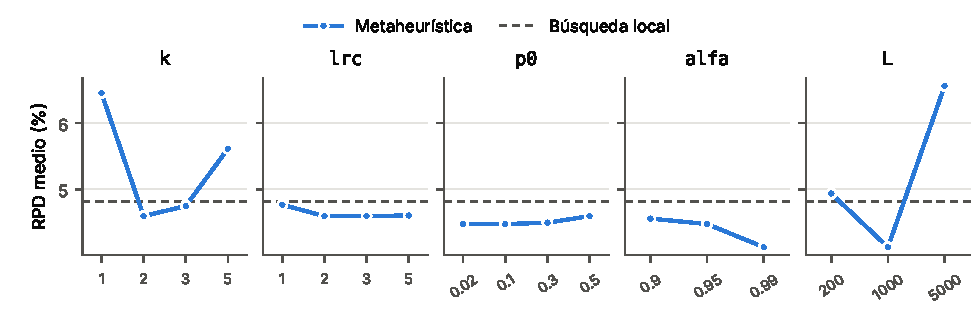
\includegraphics[width=\textwidth]{figuras/cal_temple.pdf}
\caption{Temple Simulado: RPD medio según el valor de cada parámetro.}
\end{figure}

\begin{itemize}
  \item \textbf{\cod{k} (tamaño de la vecindad): parámetro crítico.} Con $k=1$ el resultado
        (6.45) es prácticamente el del constructivo: al quitar una sola columna, la
        reparación voraz casi siempre vuelve a una solución equivalente y el temple no
        consigue moverse. Con $k=5$ (5.61) cada vecina es demasiado distinta y demasiado
        cara: se generan 138\,000 vecinas en lugar de 420\,000 y casi todas empeoran mucho.
        El mejor es $k=2$.
  \item \textbf{\cod{lrc}: basta con que no sea 1.} Con reparación determinista (1) el
        resultado es peor (4.77); entre 2, 3 y 5 la diferencia es de milésimas, es decir,
        un empate. Se conserva 2.
  \item \textbf{\cod{p0}: poco sensible.} De 0.02 a 0.3 no hay diferencias apreciables; 0.5
        es algo peor. Empezar muy caliente solo gasta tiempo aceptando empeoramientos. Se
        elige 0.1.
  \item \textbf{\cod{alfa} y \cod{L}: lo decisivo es la velocidad de enfriamiento.} Con
        $L=1000$ se recorren unas 420 temperaturas en los 5 segundos. Con $\alpha=0.99$ la
        temperatura final es $0.99^{420}\approx 0.015$ veces la inicial: un único
        enfriamiento lento que termina justo cuando se acaba el tiempo, y es lo mejor
        (4.13). Con $\alpha=0.95$ o $0.90$ el sistema se congela mucho antes y el resto del
        tiempo se va en recalentamientos (4.48 y 4.56). El caso $L=5000$ es muy instructivo:
        solo hay unas 100 temperaturas, la final es $0.99^{100}\approx 0.37$ veces la
        inicial, el sistema \emph{nunca llega a enfriarse} y el resultado (6.56) es el de la
        solución inicial: en 5 segundos no la mejora ni una vez. Con $L=200$ ocurre lo
        contrario: se enfría en un segundo y recalienta varias veces (4.94).
\end{itemize}

\textbf{Configuración elegida:} $k=2$, \cod{lrc}~$=2$, $p_0=0.1$, $\alpha=0.99$, $L=1000$. El
RPD pasa de 4.60 (base) a 4.13. La mejor solución se encuentra, de media, a los 4.1
segundos: el algoritmo sigue mejorando casi hasta el final, señal de que el enfriamiento
está bien ajustado al tiempo.

% ----------------------------------------------------------------------------
\subsection{Búsqueda Tabú}\label{sec:cal-tabu}

\begin{table}[H]
\centering
\caption{Calibración de Búsqueda Tabú. Cada fila es una etapa: RPD medio (\%) sobre las 18 ejecuciones (6 instancias $\times$ 3 semillas) de cada valor probado, con los demás parámetros fijos. En negrita, el mejor.}
\label{tab:cal-tabu}
\small
\begin{tabular}{@{}cl>{\raggedright\arraybackslash}p{10.4cm}c@{}}
\toprule
Etapa & Parámetro & Valor probado $\rightarrow$ RPD medio & Elegido \\ \midrule
1 & \texttt{tent} & 5\,$\rightarrow$\,4.215;\quad 10\,$\rightarrow$\,4.136;\quad 20\,$\rightarrow$\,\textbf{4.098};\quad 50\,$\rightarrow$\,4.280 & 20 \\
2 & \texttt{tsal} & 1\,$\rightarrow$\,\textbf{4.096};\quad 3\,$\rightarrow$\,4.098;\quad 5\,$\rightarrow$\,4.188;\quad 10\,$\rightarrow$\,4.196 & 1 \\
3 & \texttt{beta} & 0\,$\rightarrow$\,4.124;\quad 0.01\,$\rightarrow$\,\textbf{4.096};\quad 0.05\,$\rightarrow$\,4.323;\quad 0.2\,$\rightarrow$\,4.513 & 0.01 \\
4 & \texttt{reinicio} & 500\,$\rightarrow$\,4.145;\quad 2000\,$\rightarrow$\,4.096;\quad $10^6$\,$\rightarrow$\,\textbf{4.095} & $10^6$ \\
\bottomrule
\end{tabular}
\end{table}

\begin{figure}[H]\centering
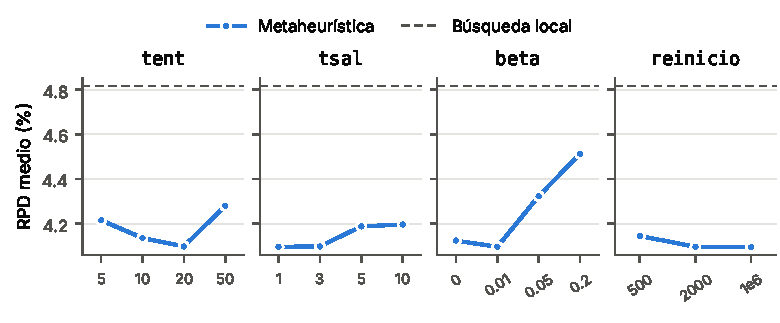
\includegraphics[width=0.85\textwidth]{figuras/cal_tabu.pdf}
\caption{Búsqueda Tabú: RPD medio según el valor de cada parámetro.}
\end{figure}

\begin{itemize}
  \item \textbf{\cod{tent} (duración tabú de entrada).} Curva en forma de U con el mínimo en
        20: con 5 la prohibición es demasiado corta (4.22) y con 50 se prohíben demasiadas
        columnas útiles (4.28).
  \item \textbf{\cod{tsal} (duración tabú de salida).} Como se había razonado en la
        sección~\ref{sec:tabu}, conviene que sea mucho más corta que la de entrada: 1 y 3
        empatan (4.10) y 5 o 10 son peores (4.19 y 4.20). Proteger durante mucho tiempo a
        las columnas recién llegadas bloquea la solución.
  \item \textbf{\cod{beta} (penalización por frecuencia).} Una penalización muy suave (0.01)
        es ligeramente mejor que ninguna (4.10 frente a 4.12, dentro del ruido), pero en
        cuanto crece empeora con claridad (4.32 y 4.51). Las frecuencias crecen sin límite
        a lo largo de la búsqueda, mientras que los valores de los movimientos son del orden
        de la unidad:
        con $\beta$ grande la penalización domina y la búsqueda deja de mirar el coste.
  \item \textbf{\cod{reinicio} (intensificación).} Volver a $s^\ast$ cada 500 iteraciones
        empeora un poco (4.15); cada 2000 o nunca da lo mismo (4.10). La intensificación por
        reinicio no aporta nada aquí.
\end{itemize}

\textbf{Configuración elegida:} \cod{tent}~$=20$, \cod{tsal}~$=1$, $\beta=0.01$, sin
reinicios. El RPD pasa de 4.14 a 4.10. \textbf{La búsqueda tabú es muy poco sensible a sus
parámetros}: entre la mejor y la peor configuración probada hay cuatro décimas. La mejor
solución aparece pronto (a los 1.6 segundos de media) y después la búsqueda se estanca, lo
que indica que su limitación no está en los parámetros sino en los movimientos.

% ----------------------------------------------------------------------------
\subsection{GRASP}\label{sec:cal-grasp}

\begin{table}[H]
\centering
\caption{Calibración de GRASP. Cada fila es una etapa: RPD medio (\%) sobre las 18 ejecuciones (6 instancias $\times$ 3 semillas) de cada valor probado, con los demás parámetros fijos. En negrita, el mejor.}
\label{tab:cal-grasp}
\small
\begin{tabular}{@{}cl>{\raggedright\arraybackslash}p{10.4cm}c@{}}
\toprule
Etapa & Parámetro & Valor probado $\rightarrow$ RPD medio & Elegido \\ \midrule
1 & \texttt{lrc} & 2\,$\rightarrow$\,4.149;\quad 3\,$\rightarrow$\,3.952;\quad 5\,$\rightarrow$\,3.729;\quad 10\,$\rightarrow$\,\textbf{3.533} & 10 \\
2 & \texttt{lamf} & 1.0\,$\rightarrow$\,4.322;\quad 0.8\,$\rightarrow$\,3.636;\quad 0.5\,$\rightarrow$\,3.533;\quad 0.2\,$\rightarrow$\,\textbf{3.519} & 0.2 \\
3 & \texttt{elite} & 5\,$\rightarrow$\,\textbf{3.441};\quad 10\,$\rightarrow$\,3.519;\quad 20\,$\rightarrow$\,3.726 & 5 \\
4 & \texttt{grent} & 2\,$\rightarrow$\,4.407;\quad 3\,$\rightarrow$\,\textbf{3.441} & 3 \\
\bottomrule
\end{tabular}
\end{table}

\begin{figure}[H]\centering
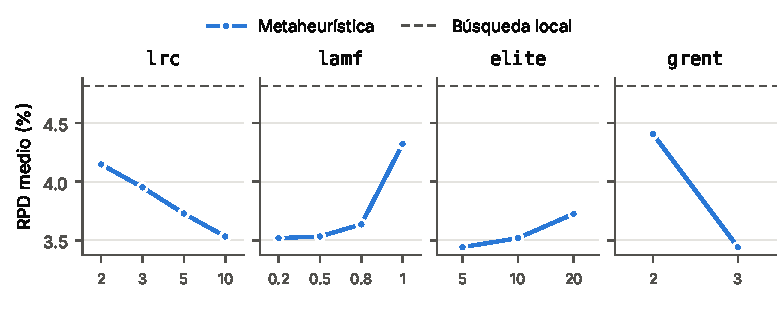
\includegraphics[width=0.85\textwidth]{figuras/cal_grasp.pdf}
\caption{GRASP: RPD medio según el valor de cada parámetro.}
\end{figure}

\begin{itemize}
  \item \textbf{\cod{lrc}.} El resultado mejora de forma continua al aumentar la lista: 4.15
        con 2 y 3.53 con 10. Más azar en la construcción da soluciones iniciales más
        variadas, y la búsqueda local se encarga de la calidad. Como gana el valor más
        grande de la lista, es posible que uno mayor sea todavía mejor: es el primer
        candidato para la segunda vuelta opcional.
  \item \textbf{\cod{lamf} (memoria): el componente más importante.} Sin memoria
        ($\lambda_f=1$, GRASP básico) el RPD es 4.32; con memoria baja a 3.52--3.64. Guiar la
        construcción hacia las columnas que aparecen en las mejores soluciones encontradas
        vale ocho décimas: es, con diferencia, el mecanismo de memoria más rentable de los
        cinco algoritmos. Entre
        $\lambda_f=0.5$ y $0.2$ hay empate.
  \item \textbf{\cod{elite}.} Mejor pequeño: 3.44 con 5 soluciones y 3.73 con 20. Un élite
        grande incluye soluciones mediocres y diluye la información.
  \item \textbf{\cod{grent}.} Con dos entornos se hacen más iteraciones (unas 600 frente a
        450) pero el resultado es mucho peor (4.41 frente a 3.44). Conviene gastar el tiempo
        en la mejora (el entorno $\D3$) y no en construir más soluciones, lo que responde a
        la pregunta que planteaban los apuntes.
\end{itemize}

\textbf{Configuración elegida:} \cod{lrc}~$=10$, $\lambda_f=0.2$, \cod{elite}~$=5$,
\cod{grent}~$=3$. El RPD pasa de 3.95 a 3.44.

% ----------------------------------------------------------------------------
\subsection{Algoritmo Genético}\label{sec:cal-genetico}

\begin{table}[H]
\centering
\caption{Calibración de Algoritmo Genético. Cada fila es una etapa: RPD medio (\%) sobre las 18 ejecuciones (6 instancias $\times$ 3 semillas) de cada valor probado, con los demás parámetros fijos. En negrita, el mejor.}
\label{tab:cal-genetico}
\small
\begin{tabular}{@{}cl>{\raggedright\arraybackslash}p{10.4cm}c@{}}
\toprule
Etapa & Parámetro & Valor probado $\rightarrow$ RPD medio & Elegido \\ \midrule
1 & \texttt{cruce} & 1\,$\rightarrow$\,\textbf{5.176};\quad 2\,$\rightarrow$\,5.436;\quad 3\,$\rightarrow$\,5.267 & 1 \\
2 & \texttt{pob} & 20\,$\rightarrow$\,\textbf{5.021};\quad 50\,$\rightarrow$\,5.176;\quad 100\,$\rightarrow$\,5.155 & 20 \\
3 & \texttt{pmut} & 0\,$\rightarrow$\,5.714;\quad 0.2\,$\rightarrow$\,5.021;\quad 0.5\,$\rightarrow$\,4.819;\quad 1.0\,$\rightarrow$\,\textbf{4.774} & 1.0 \\
4 & \texttt{nmut} & 1\,$\rightarrow$\,5.036;\quad 2\,$\rightarrow$\,4.774;\quad 5\,$\rightarrow$\,\textbf{4.613} & 5 \\
5 & \texttt{bl} & 0\,$\rightarrow$\,4.613;\quad 2\,$\rightarrow$\,\textbf{4.292} & 2 \\
\bottomrule
\end{tabular}
\end{table}

\begin{figure}[H]\centering
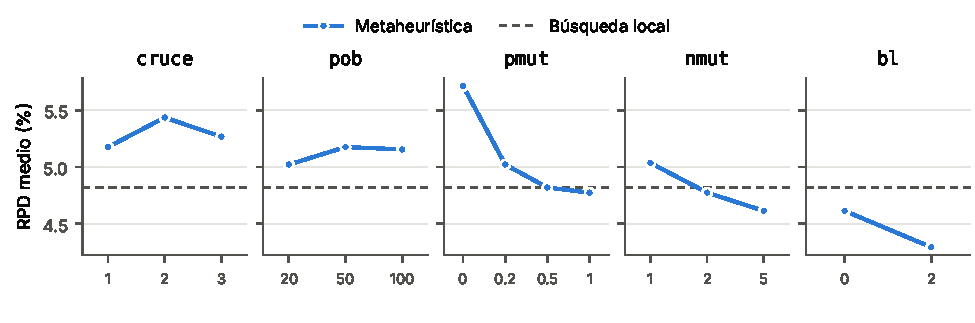
\includegraphics[width=\textwidth]{figuras/cal_genetico.pdf}
\caption{Algoritmo Genético: RPD medio según el valor de cada parámetro.}
\end{figure}

\begin{itemize}
  \item \textbf{\cod{cruce}.} El de un punto (5.18) es mejor que el ponderado (5.27) y que
        el uniforme (5.44). El cruce de un punto conserva juntos bloques enteros de columnas
        de cada progenitor, y con ellos trozos de solución que ya ``encajaban''; el uniforme
        los deshace gen a gen. Además es el más rápido (3\,400 generaciones frente a 2\,300).
  \item \textbf{\cod{pob}.} Población pequeña: 20 individuos (5.02) mejor que 50 o 100
        (5.18 y 5.16). Con el tiempo fijo, una población pequeña permite muchas más
        generaciones (12\,600 frente a 1\,100 con 100 individuos).
  \item \textbf{\cod{pmut}.} Aquí el resultado contradice la recomendación general de los
        apuntes (``probabilidad muy baja''): sin mutación el algoritmo es claramente peor
        (5.71) y mejora de forma continua hasta mutar \emph{todos} los hijos (4.77). La
        explicación es que la población es pequeña y, tras la reparación voraz, los hijos
        se parecen mucho a los padres: sin mutación la diversidad se agota enseguida. En
        este diseño la mutación (quitar columnas y reparar) hace el papel de la perturbación
        del temple y de la VNS, y es el verdadero motor de la búsqueda.
  \item \textbf{\cod{nmut}.} En la misma línea: mejor alterar 5 genes (4.61) que 1 o 2. Gana
        el extremo de la lista, así que es otro candidato para la segunda vuelta.
  \item \textbf{\cod{bl}.} Aplicar búsqueda local a los hijos (versión memética) mejora de
        4.61 a 4.29 aunque el número de generaciones se reduce a la tercera parte. Solo se
        ha probado con dos entornos; a la vista de lo que aporta $\D3$ en GRASP y VNS,
        \cod{bl}~$=3$ es el valor que la segunda vuelta opcional añade a la lista.
\end{itemize}

\textbf{Configuración elegida:} cruce de un punto, \cod{pob}~$=20$, \cod{pmut}~$=1$,
\cod{nmut}~$=5$, \cod{bl}~$=2$. El RPD pasa de 5.44 a 4.29: es el algoritmo que más gana con
la calibración, y también el que partía de la peor configuración base.

% ----------------------------------------------------------------------------
\subsection{Búsqueda en Entorno Variable}\label{sec:cal-vns}

\begin{table}[H]
\centering
\caption{Calibración de VNS. Cada fila es una etapa: RPD medio (\%) sobre las 18 ejecuciones (6 instancias $\times$ 3 semillas) de cada valor probado, con los demás parámetros fijos. En negrita, el mejor.}
\label{tab:cal-vns}
\small
\begin{tabular}{@{}cl>{\raggedright\arraybackslash}p{10.4cm}c@{}}
\toprule
Etapa & Parámetro & Valor probado $\rightarrow$ RPD medio & Elegido \\ \midrule
1 & \texttt{ja} & 1\,$\rightarrow$\,4.185;\quad 2\,$\rightarrow$\,4.228;\quad 3\,$\rightarrow$\,\textbf{3.625} & 3 \\
2 & \texttt{jb} & 2\,$\rightarrow$\,3.847;\quad 5\,$\rightarrow$\,3.625;\quad 10\,$\rightarrow$\,\textbf{3.625};\quad 20\,$\rightarrow$\,3.788 & 10 \\
3 & \texttt{lrc} & 1\,$\rightarrow$\,3.598;\quad 2\,$\rightarrow$\,3.625;\quad 3\,$\rightarrow$\,\textbf{3.585};\quad 5\,$\rightarrow$\,3.626 & 3 \\
\bottomrule
\end{tabular}
\end{table}

\begin{figure}[H]\centering
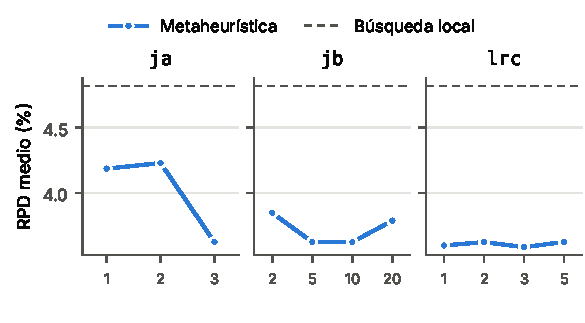
\includegraphics[width=0.68\textwidth]{figuras/cal_vns.pdf}
\caption{VNS: RPD medio según el valor de cada parámetro.}
\end{figure}

\begin{itemize}
  \item \textbf{\cod{ja} (entornos de la VND): parámetro crítico.} Con uno o dos entornos el
        RPD es 4.19 y 4.23; con los tres, 3.63, a pesar de que cada iteración es unas cien
        veces más cara (1\,700 iteraciones frente a 165\,000). Es la misma conclusión que en
        GRASP: el entorno $\D3$ es imprescindible.
  \item \textbf{\cod{jb} (tamaño máximo del salto).} Curva en U muy plana: 5 y 10 empatan
        (3.63; la media de 10 es menor por diezmilésimas, cualquiera de los dos vale), con 2
        los saltos son demasiado cortos para salir del óptimo local (3.85) y con 20
        demasiado largos (3.79).
  \item \textbf{\cod{lrc}.} Sin efecto apreciable: los cuatro valores quedan entre 3.59 y
        3.63, dentro del ruido. Se toma el de menor media.
\end{itemize}

\textbf{Configuración elegida:} $j_A=3$, $j_B=10$, \cod{lrc}~$=3$. El RPD pasa de 3.63 a
3.59: la configuración base ya era prácticamente la mejor. La VNS es, junto con la búsqueda
tabú, la metaheurística más robusta frente a sus parámetros, con la ventaja de que solo
tiene tres.

% ----------------------------------------------------------------------------
\subsection{Resumen de la calibración}

\begin{table}[H]
\centering
\caption{Configuración de partida (base) y configuración final de cada metaheurística, con su RPD medio (\%) en las instancias de calibración. En negrita, los valores que la calibración ha cambiado.}
\label{tab:config}
\begin{tabular}{@{}llcc@{}}
\toprule
Algoritmo & Parámetro & Base & Final \\ \midrule
Temple Simulado & \texttt{k} & 2 & 2 \\
 & \texttt{lrc} & 2 & 2 \\
 & \texttt{p0} & 0.5 & \textbf{0.1} \\
 & \texttt{alfa} & 0.95 & \textbf{0.99} \\
 & \texttt{L} & 1000 & 1000 \\
 & \emph{RPD medio} & \emph{4.597} & \emph{4.127} \\
\midrule
Búsqueda Tabú & \texttt{tent} & 10 & \textbf{20} \\
 & \texttt{tsal} & 3 & \textbf{1} \\
 & \texttt{beta} & 0.01 & 0.01 \\
 & \texttt{reinicio} & 2000 & \textbf{$10^6$} \\
 & \emph{RPD medio} & \emph{4.136} & \emph{4.095} \\
\midrule
GRASP & \texttt{lrc} & 3 & \textbf{10} \\
 & \texttt{lamf} & 0.5 & \textbf{0.2} \\
 & \texttt{elite} & 10 & \textbf{5} \\
 & \texttt{grent} & 3 & 3 \\
 & \emph{RPD medio} & \emph{3.952} & \emph{3.441} \\
\midrule
Algoritmo Genético & \texttt{cruce} & 2 & \textbf{1} \\
 & \texttt{pob} & 50 & \textbf{20} \\
 & \texttt{pmut} & 0.2 & \textbf{1.0} \\
 & \texttt{nmut} & 2 & \textbf{5} \\
 & \texttt{bl} & 0 & \textbf{2} \\
 & \emph{RPD medio} & \emph{5.436} & \emph{4.292} \\
\midrule
VNS & \texttt{ja} & 3 & 3 \\
 & \texttt{jb} & 5 & \textbf{10} \\
 & \texttt{lrc} & 2 & \textbf{3} \\
 & \emph{RPD medio} & \emph{3.625} & \emph{3.585} \\
\bottomrule
\end{tabular}
\end{table}


Lecciones generales de la calibración:
\begin{enumerate}
  \item \textbf{El entorno $\D3$ es el ingrediente decisivo.} Los algoritmos que lo usan en
        su búsqueda local (GRASP y VNS) son los mejores, y en ambos quitarlo cuesta entre
        seis décimas y un punto.
  \item \textbf{Los parámetros que más importan son los que fijan el tamaño del paso}
        ($k$ en el temple) \textbf{y el reparto del tiempo} ($\alpha$ y $L$ en el temple,
        el tamaño de la población en el genético). Un valor malo de estos parámetros anula
        el algoritmo: el temple con $k=1$ o con $L=5000$ no mejora al constructivo.
  \item \textbf{Los mecanismos de memoria dan resultados dispares}: la memoria de GRASP es
        muy valiosa; la penalización por frecuencia y la intensificación de la búsqueda tabú,
        casi irrelevantes.
  \item \textbf{Todas las metaheurísticas calibradas mejoran a la búsqueda local} (4.82),
        pero ninguna baja del 3.4\,\%. La sección~\ref{sec:conclusiones} analiza por qué.
\end{enumerate}

% ============================================================================
\section{Validación}\label{sec:validacion}
% ============================================================================

Fijados los parámetros (tabla~\ref{tab:config}), cada metaheurística se ha ejecutado
\emph{una sola vez} sobre las 24 instancias de \cod{Validacion\_datos/}, con las mismas 3
semillas y el mismo límite de 5 segundos: 360%
 ejecuciones.
Ningún parámetro se ha modificado después. La pregunta que responde esta sección es la de la
sección~\ref{sec:protocolo}: \emph{¿funcionan los parámetros elegidos igual de bien en
instancias que no han intervenido en su elección?}

\subsection{Calibración frente a validación}

\begin{table}[H]
\centering
\caption{Calibración frente a validación. RPD (\%) respecto del óptimo de la configuración final de cada algoritmo: media en las 6 instancias de calibración y media, desviación típica, mínimo y máximo sobre las ejecuciones en las 24 instancias de validación. Las dos últimas columnas son el número medio de columnas de la solución y el instante medio en que se encontró la mejor solución, en validación.}
\label{tab:validacion}
\begin{tabular}{@{}lrrrrrrr@{}}
\toprule
 & Calibración & \multicolumn{6}{c}{Validación} \\
\cmidrule(lr){2-2}\cmidrule(l){3-8}
Algoritmo & Media & Media & Desv. & Mín. & Máx. & Columnas & $t_{\text{mejor}}$ (s) \\ \midrule
Constructivo voraz & 6.596 & 6.448 & 0.738 & 5.167 & 7.622 & 166 & --- \\
Búsqueda local ($j_A=3$) & 4.817 & 4.665 & 0.539 & 3.816 & 6.073 & 139 & --- \\
\midrule
Temple Simulado & 4.127 & 4.067 & 0.344 & 3.131 & 4.910 & 149 & 3.75 \\
Búsqueda Tabú & 4.095 & 4.109 & 0.438 & 3.231 & 4.932 & 128 & 1.13 \\
GRASP & 3.441 & 3.448 & 0.312 & 2.639 & 4.206 & 130 & 4.32 \\
Algoritmo Genético & 4.292 & 4.275 & 0.452 & 3.112 & 5.298 & 144 & 4.51 \\
VNS & 3.585 & 3.521 & 0.451 & 2.435 & 4.499 & 124 & 3.90 \\
\bottomrule
\end{tabular}
\end{table}


\begin{figure}[H]\centering
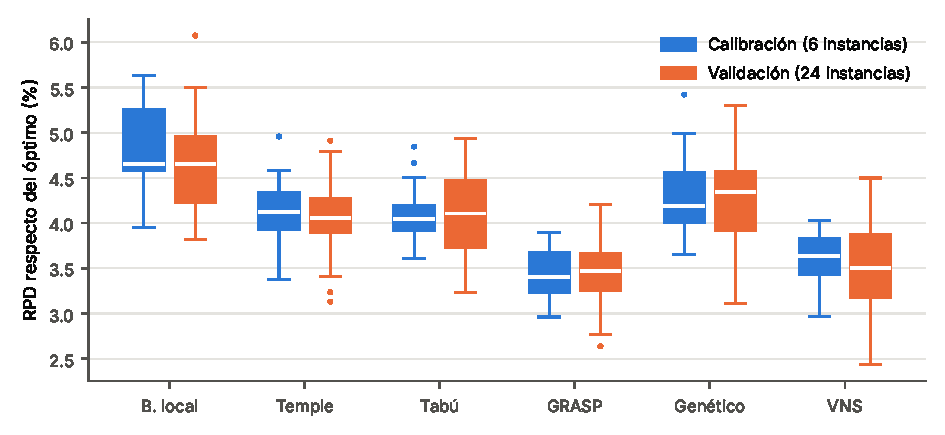
\includegraphics[width=0.86\textwidth]{figuras/validacion.pdf}
\caption{Distribución del RPD de todas las ejecuciones de la configuración final en las
instancias de calibración (18 ejecuciones por algoritmo) y de validación (72). La caja abarca
del primer al tercer cuartil; la línea blanca es la mediana.}
\label{fig:validacion}
\end{figure}

Lectura de la tabla~\ref{tab:validacion} y de la figura~\ref{fig:validacion}:
\begin{itemize}
  \item \textbf{No hay sobreajuste.} El RPD medio en validación es prácticamente igual al de
        calibración en los cinco algoritmos: la mayor diferencia es de seis centésimas
        (temple y VNS, y además a favor de la validación) y en GRASP y en la búsqueda tabú no
        llega a dos. Son diferencias menores que el propio ruido entre semillas.
  \item \textbf{La referencia confirma la lectura.} El constructivo y la búsqueda local no
        tienen nada que sobreajustar y, sin embargo, salen unas 15 centésimas mejor en las
        instancias de validación que en las de calibración: las 24 instancias de validación
        son, de media, ligerísimamente más fáciles. Las metaheurísticas se mueven menos que
        eso entre un conjunto y otro.
  \item \textbf{El orden entre algoritmos se mantiene.} En ambos conjuntos: GRASP, VNS,
        temple y tabú (empatados), genético, búsqueda local y constructivo. Lo único que
        cambia es el orden interno de la pareja temple--tabú, que están a cuatro centésimas.
  \item \textbf{La dispersión es parecida} en ambos conjuntos (figura~\ref{fig:validacion});
        en validación los extremos son algo más amplios simplemente porque hay cuatro veces
        más ejecuciones.
\end{itemize}

\begin{idea}[Conclusión de la validación]
Los parámetros elegidos con 6 instancias funcionan igual en las otras 24. La calibración es
válida para esta familia de instancias, y las cifras de validación (tabla~\ref{tab:validacion})
son las que deben usarse en el informe como estimación de la calidad de cada algoritmo.
\end{idea}

\paragraph{Una salvedad sobre el tiempo.} La validación se ejecutó en una sesión de cálculo
distinta de la calibración, en una máquina del mismo modelo que resultó en torno a un 10\,\%
más rápida (más iteraciones en los mismos 5 segundos). El efecto sobre el RPD es muy pequeño
porque al final de la ejecución todos los algoritmos mejoran ya muy despacio
(figura~\ref{fig:convergencia}), pero es una razón más para que, al repetir los experimentos,
calibración y validación se hagan seguidas en el mismo ordenador.

\subsection{Resultados por instancia}

\begin{table}[H]
\centering
\caption{Validación, instancia a instancia: valor óptimo y RPD (\%) de cada algoritmo (en las metaheurísticas, media de 3 semillas). En negrita, el mejor de cada fila.}
\label{tab:validacion-inst}
\small
\begin{tabular}{@{}lrrrrrrrr@{}}
\toprule
Instancia & Óptimo & Voraz & B. local & Temple & Tabú & GRASP & Genético & VNS \\ \midrule
SCP02 & 348.4449 & 6.69 & 4.92 & 4.34 & 4.68 & \textbf{3.48} & 4.54 & 3.73 \\
SCP03 & 360.7409 & 7.57 & 5.34 & 4.40 & 4.59 & \textbf{3.77} & 4.57 & 3.90 \\
SCP04 & 344.5675 & 5.59 & 4.23 & 4.07 & 3.65 & 3.37 & 4.17 & \textbf{3.30} \\
SCP05 & 347.3748 & 5.17 & 4.05 & 4.11 & 3.55 & 3.15 & 3.70 & \textbf{3.08} \\
SCP07 & 353.0618 & 6.09 & 4.74 & 4.20 & 4.31 & \textbf{3.69} & 4.61 & 3.84 \\
SCP08 & 351.9831 & 6.13 & 3.90 & 3.72 & 3.70 & 3.52 & 3.86 & \textbf{3.13} \\
SCP09 & 361.6024 & 6.65 & 4.44 & 4.06 & 4.10 & \textbf{3.46} & 4.22 & 3.51 \\
SCP10 & 362.9863 & 6.03 & 4.66 & 4.14 & 3.99 & \textbf{3.40} & 4.44 & 3.44 \\
SCP12 & 359.2725 & 6.07 & 4.65 & 4.00 & 4.39 & \textbf{3.27} & 4.39 & 3.47 \\
SCP13 & 350.6093 & 6.64 & 4.22 & 3.98 & 3.59 & 3.22 & 4.05 & \textbf{3.06} \\
SCP14 & 362.8942 & 7.28 & 5.15 & 3.99 & 4.21 & \textbf{3.29} & 4.27 & 3.62 \\
SCP15 & 351.7930 & 5.72 & 4.05 & 3.70 & 3.81 & \textbf{3.00} & 3.75 & 3.16 \\
SCP17 & 387.6437 & 7.22 & 5.50 & 4.34 & 4.51 & \textbf{3.80} & 4.85 & 4.36 \\
SCP18 & 379.7808 & 7.37 & 4.86 & 4.19 & 3.99 & 3.60 & 4.99 & \textbf{3.38} \\
SCP19 & 359.4288 & 5.82 & 4.87 & 3.76 & 4.04 & \textbf{3.00} & 4.17 & 3.36 \\
SCP20 & 362.8615 & 6.10 & 4.51 & 4.27 & 4.02 & 3.73 & 4.59 & \textbf{3.29} \\
SCP22 & 323.4298 & 5.97 & 4.21 & 3.30 & 3.67 & 3.13 & 3.65 & \textbf{2.80} \\
SCP23 & 363.8613 & 6.25 & 4.47 & 4.25 & 4.37 & \textbf{3.75} & 4.26 & 3.86 \\
SCP24 & 375.1956 & 7.02 & 5.21 & 3.93 & 4.52 & \textbf{3.45} & 4.55 & 3.99 \\
SCP25 & 362.9379 & 7.62 & 6.07 & 4.44 & 4.77 & 3.87 & 4.32 & \textbf{3.79} \\
SCP27 & 342.9086 & 5.72 & 3.82 & 3.88 & 3.27 & 3.45 & 3.92 & \textbf{3.04} \\
SCP28 & 321.7658 & 5.29 & 4.24 & 3.53 & 3.58 & 2.98 & 3.32 & \textbf{2.91} \\
SCP29 & 378.2595 & 7.24 & 5.07 & 4.26 & 4.80 & \textbf{3.63} & 4.52 & 4.24 \\
SCP30 & 377.9067 & 7.49 & 4.82 & 4.75 & 4.50 & \textbf{3.73} & 4.86 & 4.24 \\
\midrule
Media & & 6.45 & 4.67 & 4.07 & 4.11 & 3.45 & 4.27 & 3.52 \\
Veces mejor & & 0 & 0 & 0 & 0 & 14 & 0 & 10 \\
\bottomrule
\end{tabular}
\end{table}


La tabla~\ref{tab:validacion-inst} muestra que las conclusiones no dependen de unas pocas
instancias:
\begin{itemize}
  \item En las 24 instancias el mejor algoritmo es GRASP (14 veces) o la VNS (10 veces). La
        diferencia media entre ambos, siete centésimas a favor de GRASP, no es
        estadísticamente significativa (prueba de Wilcoxon de rangos con signo sobre las 24
        instancias, $p=0.32$): \textbf{GRASP y VNS están empatados}.
  \item La VNS es mejor que el temple en 22 de las 24 instancias y mejor que la búsqueda tabú
        en las 24; la diferencia (medio punto) sí es significativa ($p<0.001$).
  \item Temple y tabú están empatados entre sí ($p=0.53$) y ambos son algo mejores que el
        genético (dos décimas; $p<0.03$).
  \item GRASP, VNS y tabú mejoran a la búsqueda local en las 24 instancias y en sus 72
        ejecuciones; el temple, en 66 de 72; el genético, en 58 de 72.
\end{itemize}

\subsection{Evolución con el tiempo}

\begin{figure}[H]\centering
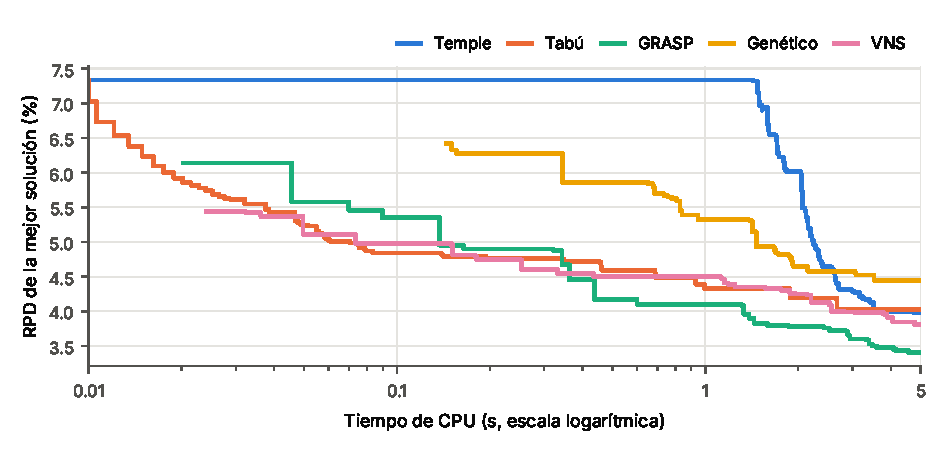
\includegraphics[width=0.86\textwidth]{figuras/convergencia.pdf}
\caption{Evolución del RPD de la mejor solución durante una ejecución de 5 segundos (instancia
SCP01, semilla 1, configuraciones finales). El eje de tiempos es logarítmico.}
\label{fig:convergencia}
\end{figure}

La figura~\ref{fig:convergencia} ilustra el comportamiento típico de cada algoritmo (es una
sola ejecución, no una media):
\begin{itemize}
  \item La \textbf{búsqueda tabú} y la \textbf{VNS} mejoran muy deprisa al principio: en una
        décima de segundo ya están en torno al 5\,\%. La tabú se estanca hacia la mitad de
        la ejecución; la VNS sigue encontrando mejoras pequeñas hasta el final.
  \item El \textbf{temple} no mejora nada durante el primer segundo y medio (fase caliente:
        acepta casi todo y la mejor solución sigue siendo la inicial) y después baja de
        golpe cuando la temperatura llega a la zona útil. Es el comportamiento esperado y
        explica por qué es tan sensible a la velocidad de enfriamiento.
  \item \textbf{GRASP} avanza a escalones cada vez más rentables: cuanto más pesa la memoria,
        mejores son las soluciones que construye. Sigue mejorando al final.
  \item El \textbf{genético} es el más lento en arrancar (tiene que construir la población),
        mejora de forma gradual durante toda la ejecución y termina por encima de los demás.
\end{itemize}

% ============================================================================
\section{Cómo compilar, ejecutar y repetir los experimentos}\label{sec:uso}
% ============================================================================

\subsection{Compilar}

Desde una terminal, dentro de la carpeta \cod{codigo/}:
\begin{verbatim}
   bash compilar.sh
\end{verbatim}
o, lo que es lo mismo, escribiendo directamente la orden que contiene ese guion:
\begin{verbatim}
   gcc -O2 -std=c99 -Wall -o scp *.c -lm
\end{verbatim}
Esto crea el ejecutable \cod{scp}. El significado de las opciones es: \cod{-O2} pide al
compilador que optimice el código (el programa va varias veces más rápido); \cod{-std=c99}
fija la versión del lenguaje; \cod{-Wall} activa los avisos; \cod{-lm} enlaza la biblioteca
matemática (por las funciones \cod{exp} y \cod{log} del temple). El código no usa nada
específico de un sistema operativo: compila igual en macOS, Linux y Windows.

\subsection{Ejecutar}

\begin{verbatim}
   ./scp FICHERO ALGORITMO [parametro=valor ...]
\end{verbatim}
donde \cod{ALGORITMO} es \cod{voraz}, \cod{local}, \cod{temple}, \cod{tabu}, \cod{grasp},
\cod{genetico} o \cod{vns}. Por ejemplo:
\begin{verbatim}
   ./scp ../datos/SCP01.dat voraz
   ./scp ../datos/SCP01.dat local
   ./scp ../datos/SCP01.dat vns
   ./scp ../datos/SCP01.dat temple tiempo=10 semilla=7
   ./scp ../datos/SCP01.dat grasp lrc=5 ver=1
\end{verbatim}
Los parámetros que no se indican toman su valor por defecto, que es el valor calibrado
(tabla~\ref{tab:config}). La tabla~\ref{tab:parametros} lista todos los nombres. Si el
programa se ejecuta sin argumentos (por ejemplo, con el botón de ejecutar de un editor),
pregunta el fichero y el algoritmo por teclado.

\begin{table}[H]
\centering
\caption{Parámetros que admite el programa en la línea de órdenes.}
\label{tab:parametros}
\small\setlength{\tabcolsep}{4.5pt}
\begin{tabular}{@{}llp{7.6cm}@{}}
\toprule
Ámbito & Parámetro & Significado \\ \midrule
General & \cod{tiempo} & límite de tiempo de CPU en segundos (5 por defecto) \\
        & \cod{semilla} & semilla de los números aleatorios (1 por defecto) \\
        & \cod{ver} & con \cod{ver=1} escribe las columnas de la solución \\
        & \cod{traza} & con \cod{traza=1} escribe cada mejora y el instante en que se produce \\
Voraz y local & \cod{criterio} & criterio voraz: 1, 2 o 3 \\
        & \cod{entornos} & $j_A$ de la búsqueda local: 1, 2 o 3 \\
Temple & \cod{k}, \cod{lrc}, \cod{p0}, \cod{alfa}, \cod{L} & sección~\ref{sec:temple} \\
Tabú & \cod{tent}, \cod{tsal}, \cod{beta}, \cod{reinicio} & sección~\ref{sec:tabu} \\
GRASP & \cod{lrc}, \cod{lam0}, \cod{lamf}, \cod{elite}, \cod{grent} & sección~\ref{sec:grasp} \\
Genético & \cod{pob}, \cod{cruce}, \cod{pmut}, \cod{nmut}, \cod{bl} & sección~\ref{sec:genetico} \\
VNS & \cod{jb}, \cod{ja}, \cod{lrc} & sección~\ref{sec:vns} \\
\bottomrule
\end{tabular}
\end{table}

La salida tiene este aspecto:
\begin{verbatim}
   Instancia : ../datos/SCP01.dat  (m = 500 filas, n = 10000 columnas)
   Algoritmo : local   (semilla 1, limite 5.0 s)
   Coste     : 389.4609
   Columnas  : 144
   Factible  : SI
   RESULTADO;../datos/SCP01.dat;local;1;389.4609;144;0.028;0.028;0;1
\end{verbatim}
La última línea repite la información en un formato fácil de leer por otro programa (lo usan
los guiones de experimentos): fichero, algoritmo, semilla, coste, número de columnas,
segundos hasta la mejor solución, segundos totales, iteraciones y un 1 si la solución ha
superado la comprobación de factibilidad.

\subsection{Repetir los experimentos en otro ordenador}

La carpeta \cod{experimentos/} contiene todo lo necesario para repetir la calibración y la
validación. La forma más cómoda es un único guion que lo hace todo por orden:
\begin{verbatim}
   cd experimentos
   bash repetir_todo.sh
\end{verbatim}
Este guion compila el programa, guarda los resultados anteriores en una carpeta aparte (no
borra nada), ejecuta todos los experimentos, genera las
tablas y figuras y compila la memoria. Equivale a lanzar a mano, uno tras otro:
\begin{verbatim}
   python3 basicos.py          (constructivo y busqueda local; unos segundos)
   python3 calibrar.py         (calibracion: 1008 ejecuciones de 5 s)
   python3 validar.py          (validacion: 360 ejecuciones de 5 s)
   python3 trazas.py           (curvas de convergencia; medio minuto)
   python3 estructura.py       (comparacion con la solucion optima; 2-3 minutos)
   python3 generar_tablas.py   (tablas y figuras de la memoria)
\end{verbatim}
\begin{itemize}
  \item \textbf{Duración.} La calibración son 84 minutos de cálculo y la validación 30, que se
        reparten entre las ejecuciones que se lancen a la vez: con 4 a la vez, unos 20 y 8
        minutos. El número de ejecuciones simultáneas se fija con la variable de entorno
        \cod{PROCESOS} (por ejemplo \cod{PROCESOS=4 python3 calibrar.py}); por defecto son 2,
        y \cod{repetir\_todo.sh} lo ajusta al número de núcleos del ordenador. No conviene
        poner más que núcleos haya.
  \item \textbf{Segunda vuelta.} \cod{VUELTAS=2 python3 calibrar.py} añade la segunda vuelta de
        la sección~\ref{sec:ofat} (aproximadamente el doble de tiempo).
  \item \textbf{Reanudar.} \cod{calibrar.py} y \cod{validar.py} guardan cada ejecución en
        cuanto termina. Si se interrumpen, al volver a lanzarlos continúan donde lo dejaron.
        Por la misma razón, si ya existe un fichero de resultados \emph{no} repiten lo que
        contiene: para recalcular desde cero hay que apartar antes
        \cod{resultados\_calibracion.csv} y \cod{resultados\_validacion.csv} (es lo que hace
        \cod{repetir\_todo.sh}).
  \item \textbf{Requisitos.} Python~3; \cod{generar\_tablas.py} usa además \cod{matplotlib}
        para las figuras (si no está instalado, genera solo las tablas).
  \item \textbf{Las cifras cambiarán algo.} En 5 segundos un procesador más rápido hace más
        iteraciones. Lo importante es que calibración y validación se ejecuten en el mismo
        ordenador. Si la nueva calibración elige otros valores (fichero
        \cod{decisiones.json}), conviene copiarlos a los valores por defecto del programa
        (función \cod{parametros\_por\_defecto} de \cod{main.c}) y revisar los comentarios de
        la sección~\ref{sec:calibracion}.
  \item \cod{calcular\_optimos.py} recalcula los óptimos (necesita \cod{numpy} y \cod{scipy}).
        No hace falta ejecutarlo: los valores están en \cod{optimos.csv}.
\end{itemize}

Ficheros de resultados que acompañan a la memoria:
\begin{center}
\small
\begin{tabular}{@{}lp{10.2cm}@{}}
\toprule
Fichero & Contenido \\ \midrule
\cod{optimos.csv} & valor óptimo de las 30 instancias \\
\cod{resultados\_basicos.csv} & constructivo y búsqueda local en las 30 instancias \\
\cod{resultados\_calibracion.csv} & todas las ejecuciones de la calibración, una por línea \\
\cod{decisiones.json} & etapas de la calibración, valor elegido en cada una y configuración final \\
\cod{resultados\_validacion.csv} & todas las ejecuciones de la validación \\
\cod{resultados\_trazas.csv} & evolución de la mejor solución con el tiempo \\
\cod{resultados\_estructura.csv} & columnas de cada solución compartidas con la óptima \\
\cod{optimos\_soluciones.csv} & columnas de la solución óptima de cada instancia \\
\cod{calibracion.log}, \cod{validacion.log} & lo que escribieron los guiones por pantalla \\
\bottomrule
\end{tabular}
\end{center}

% ============================================================================
\section{Conclusiones}\label{sec:conclusiones}
% ============================================================================

\subsection{Qué se ha hecho}

Se han implementado en C, sobre una base común de estructuras de datos, un algoritmo
constructivo, una búsqueda local con tres estructuras de entornos y cinco metaheurísticas que
siguen los esquemas de los apuntes. Sus 21 parámetros se han calibrado con un procedimiento
de un factor cada vez sobre 6 instancias, y las configuraciones resultantes se han validado
sobre otras 24. En total, 1548%
 ejecuciones, todas con solución
factible verificada de forma independiente.

\subsection{Resultados}

\begin{center}
\begin{tabular}{@{}lcl@{}}
\toprule
Algoritmo & RPD en validación & Tiempo \\ \midrule
Constructivo voraz (cociente) & 6.45\,\% & 0.01 s \\
Búsqueda local ($\D1,\D2,\D3$) & 4.67\,\% & 0.03 s \\
Algoritmo Genético & 4.28\,\% & 5 s \\
Búsqueda Tabú & 4.11\,\% & 5 s \\
Temple Simulado & 4.07\,\% & 5 s \\
VNS & 3.52\,\% & 5 s \\
GRASP & 3.45\,\% & 5 s \\
\bottomrule
\end{tabular}
\end{center}

\begin{itemize}
  \item Las cinco metaheurísticas mejoran a la búsqueda local, y la validación confirma que
        los parámetros elegidos no están sobreajustados.
  \item \textbf{GRASP (con memoria) y VNS son las mejores}, empatadas entre sí, medio punto
        por delante de temple y tabú. Las dos tienen algo en común: aplican la búsqueda
        local completa (con el entorno $\D3$) a muchas soluciones distintas.
  \item El \textbf{genético} es el más flojo; en la forma calibrada funciona, de hecho, como
        una búsqueda por perturbación (muta todos los hijos) más que como un algoritmo
        evolutivo.
  \item La ganancia de las metaheurísticas sobre la búsqueda local es modesta: entre 0.4 y
        1.2 puntos a cambio de 200 veces más tiempo.
\end{itemize}

\subsection{Por qué ninguna baja del 3.4\,\%}\label{sec:barrera}

Este es el resultado más llamativo y merece una explicación. La tabla~\ref{tab:estructura}
compara las soluciones de cada algoritmo con la solución óptima, columna a columna.

\begin{table}[H]
\centering
\caption{Estructura de las soluciones en las 6 instancias de calibración (semilla 1): RPD, número de columnas y cuántas de ellas pertenecen también a la solución óptima, que tiene 50 columnas. Medias de las 6 instancias.}
\label{tab:estructura}
\begin{tabular}{@{}lrrr@{}}
\toprule
Solución & RPD (\%) & Columnas & Comunes con la óptima \\ \midrule
Voraz, criterio 2 (mayor cobertura) & 33.43 & 49.2 & 27.2 \\
Voraz, criterio 3 (cociente) & 6.60 & 167.3 & 3.0 \\
Búsqueda local ($j_A=3$) & 4.82 & 141.7 & 3.2 \\
\midrule
Temple Simulado & 4.14 & 148.3 & 4.3 \\
Búsqueda Tabú & 4.02 & 124.5 & 4.0 \\
GRASP & 3.27 & 128.3 & 5.3 \\
Algoritmo Genético & 4.33 & 145.0 & 5.3 \\
VNS & 3.68 & 128.8 & 2.7 \\
Solución óptima & 0.00 & 50.0 & 50.0 \\
\bottomrule
\end{tabular}
\end{table}


\begin{itemize}
  \item La solución óptima usa \textbf{50 columnas grandes}. Las soluciones de todos los
        heurísticos usan entre 125 y 170 \textbf{columnas pequeñas y baratas}, y solo
        comparten con la óptima entre 3 y 5 columnas. No están ``cerca del óptimo con algún
        detalle por pulir'': son soluciones de otra clase, que casualmente cuestan casi lo
        mismo.
  \item El voraz de mayor cobertura (criterio 2) sí encuentra más de la mitad de las columnas
        óptimas (27 de 50), pero completa la solución con columnas grandes equivocadas y
        carísimas, y queda un 33\,\% por encima.
  \item Hay, por tanto, \textbf{dos familias de soluciones}: muchas columnas pequeñas (a un
        3--6\,\% del óptimo) y pocas columnas grandes (donde está el óptimo, pero también
        soluciones muy malas). Para pasar de la primera a la segunda hay que cambiar más de
        cien columnas, y los pasos intermedios son peores: tener ya la mitad de las columnas
        óptimas no garantiza nada, como muestra el criterio 2.
  \item El criterio del cociente coste/cobertura, que es el que guía la construcción, las
        reparaciones y las perturbaciones de todos los algoritmos, empuja siempre hacia la
        primera familia, porque las columnas diminutas y casi gratuitas tienen mejor
        cociente que las columnas de la solución óptima.
\end{itemize}

\begin{idea}[Interpretación]
Las cinco metaheurísticas exploran bien la familia de soluciones de columnas pequeñas (por
eso mejoran a la búsqueda local y son robustas en validación), pero ninguno de sus
mecanismos de escape (aceptar empeoramientos, prohibir movimientos, reiniciar, cruzar,
saltar) es capaz de dar el salto a la otra familia en 5 segundos. No es un problema de
calibración: la calibración mueve los resultados unas décimas, y la distancia al óptimo es
de más de tres puntos.
\end{idea}

Como se indicó en la sección~\ref{sec:optimos}, estas instancias tienen además una propiedad
especial (la relajación lineal ya da el óptimo entero) que las hace fáciles para un método
exacto. Un heurístico que usara la información de la relajación lineal o de sus variables
duales para elegir columnas tendría aquí una gran ventaja, pero eso queda fuera de las
metaheurísticas que pide la práctica.

\subsection{Limitaciones y posibles mejoras}

\begin{itemize}
  \item \textbf{Calibración de una vuelta.} No capta interacciones entre parámetros, y en
        varios parámetros ganó un valor extremo de su lista (por ejemplo \cod{alfa} del
        temple, \cod{lrc} y \cod{elite} de GRASP, o \cod{pob}, \cod{nmut} y \cod{bl} del
        genético), de modo que el mejor valor podría estar más allá. La segunda vuelta
        opcional de \cod{calibrar.py} está pensada para eso.
  \item \textbf{Tres semillas.} Suficientes para elegir parámetros con diferencias claras,
        justas para los empates. Para el informe convendría ejecutar las configuraciones
        finales con más semillas (por ejemplo 10) y aplicar pruebas estadísticas a todas las
        comparaciones.
  \item \textbf{Un único límite de tiempo.} Los parámetros son los mejores para 5 segundos.
        La figura~\ref{fig:convergencia} indica que GRASP, VNS y temple todavía mejoran al
        final, así que con más tiempo las diferencias podrían cambiar.
  \item \textbf{Una única familia de instancias.} Todas tienen el mismo tamaño y estructura;
        las conclusiones no se pueden extender sin más a otros problemas de cubrimiento.
  \item \textbf{Movimientos.} La explicación de la sección~\ref{sec:barrera} sugiere dónde
        buscar mejoras: construcciones o reparaciones que no usen solo el cociente (por
        ejemplo, alternándolo con el criterio de mayor cobertura) para sembrar soluciones de
        la otra familia.
\end{itemize}

% ============================================================================
%  Bibliografia. Todos los enlaces son de acceso libre y gratuito, sin
%  suscripcion ni registro.
% ============================================================================
\begin{thebibliography}{99}
\addcontentsline{toc}{section}{Referencias}

\bibitem{apuntes}
Transparencias de la asignatura \emph{Técnicas Avanzadas de Optimización} (Departamento de
Estadística e Investigación Operativa, Universidad Complutense de Madrid): ``Teoría de la
complejidad. Heurísticas y metaheurísticas'', ``Algunas heurísticas clásicas'', ``Temple
Simulado, Búsqueda Tabú, GRASP y Algoritmos Genéticos'' y ``Búsqueda en Entorno Variable.
Aplicación al doble TSP con múltiples pilas'' (G.~Tirado Domínguez). Material del curso. De
ellas se han tomado las definiciones y los esquemas de los algoritmos.

\bibitem{yanez}
J.~Yáñez. \emph{Metaheurísticas}. Apuntes de Ingeniería Matemática (Optimización y
Simulación), Universidad Complutense de Madrid. Material del curso. Capítulos 2 (algoritmos
voraces e iterativos), 3 (temple simulado), 4 (algoritmos genéticos) y 5 (búsqueda tabú).

\bibitem{orlib}
J.~E.~Beasley. \emph{OR-Library: Set covering}. Descripción de las instancias de prueba del
problema de cubrimiento y de su formato de fichero.\\
\url{http://people.brunel.ac.uk/~mastjjb/jeb/orlib/scpinfo.html}

\bibitem{luke}
S.~Luke. \emph{Essentials of Metaheuristics}, 2.ª edición. Lulu, 2013. Libro completo
disponible gratuitamente en la página del autor.\\
\url{https://cs.gmu.edu/~sean/book/metaheuristics/}

\bibitem{bertsimas}
D.~Bertsimas y J.~Tsitsiklis. Simulated Annealing. En \emph{Probability and Algorithms},
cap.~2, págs.~17--30. National Academies Press, 1992. Lectura en línea y PDF gratuitos.\\
\url{https://www.nationalacademies.org/read/2026/chapter/3}

\bibitem{glover}
F.~Glover, E.~Taillard y D.~de Werra. A user's guide to tabu search. \emph{Annals of
Operations Research} 41 (1993), 3--28. Copia en la página de F.~Glover (Universidad de
Colorado).\\
\url{https://leeds-faculty.colorado.edu/glover/fred%20pubs/228%20-%20TS%20-%20Users%20Guide%201993.pdf}

\bibitem{resende}
M.~G.~C.~Resende y C.~C.~Ribeiro. Greedy randomized adaptive search procedures. En
\emph{Handbook of Metaheuristics} (F.~Glover y G.~Kochenberger, eds.), págs.~219--249.
Kluwer, 2002. PDF del capítulo en la página del autor.\\
\url{https://mauricio.resende.info/abstracts/sgrasp-hmetah.html}

\bibitem{vnsbasics}
P.~Hansen, N.~Mladenović, R.~Todosijević y S.~Hanafi. Variable neighborhood search: basics
and variants. \emph{EURO Journal on Computational Optimization} 5(3) (2017), 423--454.
Revista de acceso abierto.\\
\url{https://doaj.org/article/5d1a1060d0b449c0ad56b79a04b69e53}

\bibitem{irace}
M.~López-Ibáñez, J.~Dubois-Lacoste, L.~Pérez Cáceres, M.~Birattari y T.~Stützle. The irace
package: Iterated racing for automatic algorithm configuration. \emph{Operations Research
Perspectives} 3 (2016), 43--58. Revista de acceso abierto.\\
\url{https://doi.org/10.1016/j.orp.2016.09.002}

\bibitem{kordalewski}
D.~Kordalewski. New Greedy Heuristics for Approximating Set Cover and Set Packing.
arXiv:1305.3584, 2013. La sección~2.3 describe el voraz estándar del cubrimiento y su
garantía de aproximación.\\
\url{https://arxiv.org/pdf/1305.3584}

\bibitem{tayebi}
D.~Tayebi, S.~Ray y D.~Ajwani. An Improved Genetic Algorithm for Set Cover using Rosenthal
Potential. \emph{Proceedings of the 19th Conference on Computer Science and Intelligence
Systems (FedCSIS)}, ACSIS vol.~39 (2024), 689--694. Acceso abierto.\\
\url{https://www.annals-csis.org/Volume_39/drp/pdf/7060.pdf}

\bibitem{scipymilp}
SciPy. Documentación de \texttt{scipy.optimize.milp}, función de programación lineal entera
que utiliza el resolutor libre HiGHS.\\
\url{https://docs.scipy.org/doc/scipy/reference/generated/scipy.optimize.milp.html}

\end{thebibliography}

\noindent{\small Todas las fuentes externas citadas son de acceso libre y gratuito, sin pago,
registro ni suscripción. Enlaces comprobados el 14 de noviembre de 2026.}



\appendix
% ============================================================================
\section{Código completo}\label{sec:codigo}
% ============================================================================

Se reproduce a continuación el código íntegro del programa, tal como está en la carpeta
\cod{codigo/}. Cada línea lleva a su derecha un comentario que explica qué hace. Los
comentarios del código están escritos sin tildes para evitar problemas de codificación al
abrir los ficheros en distintos sistemas.

\newcommand{\listado}[2]{\subsection{\texttt{#1}}\lstinputlisting{../codigo/#2}}
\listado{scp.h}{scp.h}
\listado{base.c}{base.c}
\listado{constructivo.c}{constructivo.c}
\listado{busqueda\_local.c}{busqueda_local.c}
\listado{temple.c}{temple.c}
\listado{tabu.c}{tabu.c}
\listado{grasp.c}{grasp.c}
\listado{genetico.c}{genetico.c}
\listado{vns.c}{vns.c}
\listado{main.c}{main.c}


\end{document}
